\documentclass[a4paper,12pt]{article}

\usepackage{vntex}
\usepackage[a4paper,margin=2.5cm]{geometry}
\usepackage{graphicx}
\usepackage{float}
\usepackage{array}
\usepackage{tabularx}
\usepackage{longtable}
\usepackage{booktabs}
\usepackage{multirow}
\usepackage{amsmath}
\usepackage{fancyhdr}
\usepackage{lastpage}
\usepackage{xcolor}
\usepackage{listings}
\usepackage{hyperref}
\usepackage{setspace}
\usepackage{enumitem}
\usepackage[framemethod=tikz]{mdframed}


\usepackage{makecell}


\hypersetup{
    colorlinks=true,
    linkcolor=black,
    urlcolor=blue,
    citecolor=black
}

\setstretch{1.25}
\setlength{\headheight}{40pt}

\pagestyle{fancy}
\fancyhf{}
\fancyhead[L]{
    \begin{tabular}{l}
        \textbf{TRƯỜNG ĐẠI HỌC SÀI GÒN}\\
        \textbf{KHOA CÔNG NGHỆ THÔNG TIN}
    \end{tabular}
}
\fancyfoot[L]{\footnotesize Đồ án môn học -- Trang web mạng xã hội Fookbase}
\fancyfoot[R]{\footnotesize Trang \thepage/\pageref{LastPage}}
\renewcommand{\headrulewidth}{0.3pt}
\renewcommand{\footrulewidth}{0.3pt}

\definecolor{dkgreen}{rgb}{0,0.5,0}
\definecolor{gray}{rgb}{0.5,0.5,0.5}
\definecolor{mauve}{rgb}{0.58,0,0.82}
\definecolor{lightgray}{rgb}{0.97,0.97,0.97}

\lstset{
    backgroundcolor=\color{lightgray},
    basicstyle=\ttfamily\small,
    breaklines=true,
    frame=single,
    numbers=left,
    numberstyle=\tiny\color{gray},
    showstringspaces=false,
    keywordstyle=\color{blue},
    commentstyle=\color{dkgreen},
    stringstyle=\color{mauve},
    tabsize=2
}

\begin{document}

% ========================= TRANG BÌA =========================
\begin{titlepage}
\begin{center}
    \textbf{\footnotesize TRƯỜNG ĐẠI HỌC SÀI GÒN}\\
    \textbf{\footnotesize KHOA CÔNG NGHỆ THÔNG TIN}
\end{center}

\vspace{1cm}

\begin{figure}[H]
\centering
% Thay logo nếu có

\includegraphics[width=3cm]{logoITSGU.png}
\end{figure}

\vspace{1cm}
\begin{center}
{\color{blue}
\begin{tabular}{c}
    \multicolumn{1}{l}{\textbf{\Large NGÔN NGỮ LẬP TRÌNH C\#}}\\
    \\
    \hline
    \\
    \multicolumn{1}{c}{\textbf{\Large XÂY DỰNG TRANG WEB MẠNG XÃ HỘI}}\\
    \\
    \multicolumn{1}{c}{\textbf{\Huge FOOKBASE}}\\
    \\
    \hline
\end{tabular}
}
\end{center}

\vspace{3cm}

\begin{table}[H]
\centering
{\color{blue}
\begin{tabular}{r l l}
    & GVHD: & Từ Lãng Phiêu \\
    & SV:   & Lâm Thái Yến Nhi -- 3123410076 \\
    &       & Châu Hải Đăng -- 3123410076 \\
    &       & Lê Thắng Minh -- 3123410076 \\
    &       & Trần Đình Khánh Dư -- 3123410063 \\
    &       & Nguyễn Hải Đăng -- 3123410076 \\
\end{tabular}
}
\end{table}
\vfill

\begin{center}
    {\footnotesize TP. Hồ Chí Minh, năm 2026}
\end{center}
\end{titlepage}

% ========================= MỤC LỤC =========================
\tableofcontents
\newpage

% ========================= GIỚI THIỆU =========================
\section{Lời giới thiệu}

Trong bối cảnh các nền tảng mạng xã hội ngày càng phát triển mạnh mẽ, nhu cầu xây dựng một hệ thống cho phép người dùng kết nối, chia sẻ thông tin, tương tác và trao đổi trực tuyến ngày càng trở nên quan trọng. Xuất phát từ thực tế đó, nhóm thực hiện đề tài xây dựng trang web mạng xã hội mang tên \textbf{Fookbase}, định hướng phát triển theo mô hình tương tự Facebook với các chức năng cốt lõi như đăng ký, đăng nhập, tạo bài viết, tương tác bài viết, bình luận, quản lý hồ sơ cá nhân, kết bạn và nhận thông báo.

Mục tiêu của đề tài không chỉ dừng lại ở việc xây dựng một giao diện có thể sử dụng được, mà còn tập trung vào việc mô tả rõ ràng luồng hoạt động của toàn hệ thống, bao gồm cách người dùng thao tác trên giao diện, cách frontend gửi yêu cầu đến backend thông qua API, cách backend xử lý nghiệp vụ, truy vấn cơ sở dữ liệu và trả kết quả về cho người dùng. Việc mô tả chi tiết các luồng hoạt động này giúp làm rõ kiến trúc của hệ thống, tăng tính trực quan trong quá trình báo cáo, đồng thời hỗ trợ kiểm thử và bảo trì về sau.

Bên cạnh đó, báo cáo cũng trình bày phần hiển thị kết quả giao diện của trang web sau khi hoàn thiện, các chức năng chính đã xây dựng, và một số đoạn mã kiểm thử nhằm chứng minh hệ thống hoạt động đúng theo yêu cầu đặt ra. Qua đề tài này, nhóm mong muốn vận dụng kiến thức về phát triển web, thiết kế API, xử lý dữ liệu và tổ chức hệ thống phần mềm để tạo ra một sản phẩm có tính ứng dụng thực tế, có thể tiếp tục mở rộng trong tương lai.

\section{Mục tiêu và phạm vi đề tài}

\subsection{Mục tiêu đề tài}
Đề tài hướng đến việc xây dựng một trang web mạng xã hội có tên \textbf{Fookbase} với các chức năng cơ bản của một hệ thống mạng xã hội hiện đại, bao gồm:
\begin{itemize}
    \item Cho phép người dùng đăng ký, đăng nhập và đăng xuất tài khoản.
    \item Quản lý hồ sơ cá nhân và cập nhật thông tin người dùng.
    \item Đăng bài viết, chỉnh sửa bài viết, xóa bài viết.
    \item Tương tác với bài viết thông qua lượt thích, bình luận và chia sẻ.
    \item Hỗ trợ tìm kiếm người dùng, kết bạn và quản lý danh sách bạn bè.
    \item Hiển thị bảng tin (news feed) theo thời gian thực hoặc gần thời gian thực.
    \item Kết nối frontend với backend thông qua API để xử lý dữ liệu.
\end{itemize}

\subsection{Phạm vi đề tài}
Trong khuôn khổ báo cáo này, nhóm tập trung vào:
\begin{itemize}
    \item Thiết kế và xây dựng giao diện người dùng của hệ thống.
    \item Xây dựng các API phục vụ chức năng chính của hệ thống.
    \item Tổ chức dữ liệu và xử lý nghiệp vụ ở phía máy chủ.
    \item Mô tả chi tiết luồng hoạt động của website.
    \item Thực hiện kiểm thử một số chức năng tiêu biểu.
\end{itemize}

\section{Bảng phân chia công việc}

\begin{table}[H]
\centering
\caption{Phân chia công việc trong nhóm}
\begin{tabular}{|c|l|c|}
\hline
\textbf{STT} & \textbf{Thành viên} & \textbf{Tỉ lệ} \\
\hline
1 & Lâm Thái Yến Nhi & 20\% \\
2 & Châu Hải Đăng & 20\% \\
3 & Lê Thắng Minh & 20\% \\
4 & Trần Đình Khánh Dư & 20\% \\
5 & Nguyễn Hải Đăng & 20\% \\
\hline
\end{tabular}
\end{table}

% ========================= TỔNG QUAN HỆ THỐNG =========================
\section{Tổng quan hệ thống Fookbase}

\subsection{Mô tả hệ thống}
Fookbase là một hệ thống mạng xã hội được xây dựng nhằm mô phỏng và phát triển các chức năng phổ biến của Facebook. Hệ thống cho phép người dùng đăng ký, đăng nhập, hoàn thiện hồ sơ cá nhân, kết bạn, đăng bài viết, bình luận, thả cảm xúc, tạo story, lưu bài viết, nhận thông báo, nhắn tin và tương tác với những người dùng khác. Phía client của hệ thống gồm ứng dụng web chạy trên trình duyệt và ứng dụng mobile chạy trên điện thoại.

Hệ thống được xây dựng theo mô hình client-server với kiến trúc nhiều dịch vụ. Frontend web và mobile sẽ gửi yêu cầu đến backend thông qua API khi người dùng thực hiện các thao tác như đăng nhập, tạo bài viết, gửi lời mời kết bạn, nhắn tin hoặc xem thông báo. Phía backend của Fookbase gồm hai hệ thống chính phối hợp với nhau: backend ASP.NET Core (C sharp) phụ trách các chức năng như bài viết, bình luận, story, thông báo, lưu bài viết, báo cáo nội dung, đánh giá ứng dụng, quản trị và game; backend Spring Boot (Java) phụ trách xác thực người dùng, hồ sơ cá nhân, quan hệ bạn bè, danh bạ và nhắn tin. Hai backend làm việc với các cơ sở dữ liệu và dịch vụ hỗ trợ riêng, đồng thời trao đổi dữ liệu để đảm bảo hệ thống hoạt động đồng bộ. Sau khi xử lý nghiệp vụ và truy xuất dữ liệu, backend sẽ trả kết quả về cho client để cập nhật giao diện; với các chức năng thời gian thực như nhắn tin và thông báo, hệ thống sử dụng kết nối realtime để cập nhật ngay cho người dùng.




\subsection{Các thành phần chính của hệ thống}
\begin{itemize}
    \item \textbf{Frontend web:} chịu trách nhiệm hiển thị giao diện trên trình duyệt, nhận thao tác người dùng và gửi yêu cầu đến các backend để xử lý các chức năng như bài viết, story, hồ sơ, bạn bè, thông báo, game và quản trị.
     \item \textbf{Frontend mobile:} cung cấp giao diện trên thiết bị di động, hỗ trợ các chức năng chính như đăng nhập, hoàn thiện hồ sơ, danh bạ, kết bạn, nhắn tin cá nhân và nhóm.
    \item \textbf{Backend ASP.NET Core (C#):}  xử lý các chức năng liên quan đến bài viết, bình luận, cảm xúc, story, lưu bài viết, thông báo, báo cáo nội dung, đánh giá ứng dụng, quản trị và game thời gian thực.
    \item \textbf{Backend Spring Boot (Java):}  xử lý xác thực người dùng, đăng ký, đăng nhập, OTP, hồ sơ cá nhân, quan hệ bạn bè, danh bạ, nhắn tin và quản lý hội thoại.
    \item \textbf{Cơ sở dữ liệu và dịch vụ hỗ trợ:} PostgreSQL dùng để lưu dữ liệu phía backend C#, MySQL dùng để lưu dữ liệu phía backend Java; ngoài ra hệ thống còn sử dụng Redis, RabbitMQ và các dịch vụ lưu trữ media để hỗ trợ realtime, đồng bộ dữ liệu và quản lý tệp.
    \item \textbf{Cơ chế giao tiếp:} frontend web và mobile giao tiếp với hai backend thông qua REST API dùng HTTP/HTTPS; các chức năng cần cập nhật tức thời như nhắn tin, thông báo và game sử dụng kết nối realtime như WebSocket/SignalR.
\end{itemize}

\subsection{Cấu trúc dự án}
Fookbase được tổ chức theo hướng tách biệt từng thành phần để dễ phát triển và bảo trì. Mỗi khối (frontend web, frontend mobile, backend C\#, backend Java) có cấu trúc thư mục riêng, tập trung theo chức năng, sau đó kết nối với nhau qua API.

\begin{figure}[H]
    \centering
    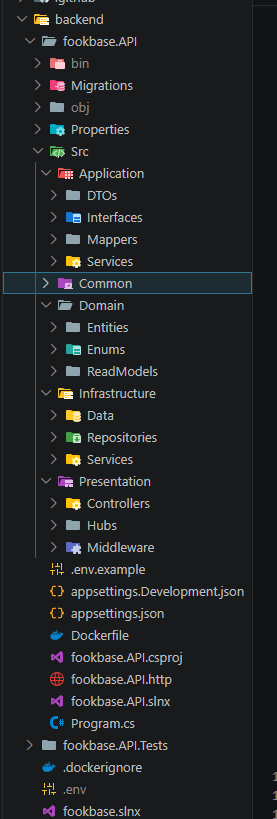
\includegraphics[width=0.9\textwidth]{images/cautrucbecs.png}
    \caption{Cấu trúc backend C\#}
\end{figure}

\begin{figure}[H]
    \centering
    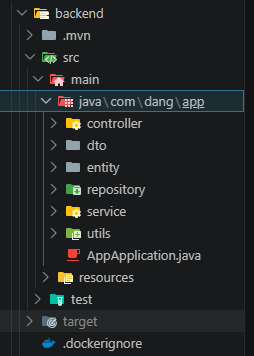
\includegraphics[width=0.9\textwidth]{images/cautrucbejava.png}
    \caption{Cấu trúc backend Java}
\end{figure}

\begin{figure}[H]
    \centering
    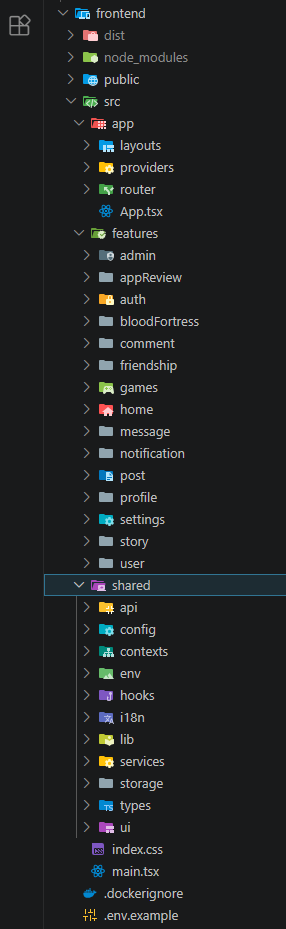
\includegraphics[width=0.9\textwidth]{images/cautrucfecs.png}
    \caption{Cấu trúc frontend C\# (web)}
\end{figure}

\begin{figure}[H]
    \centering
    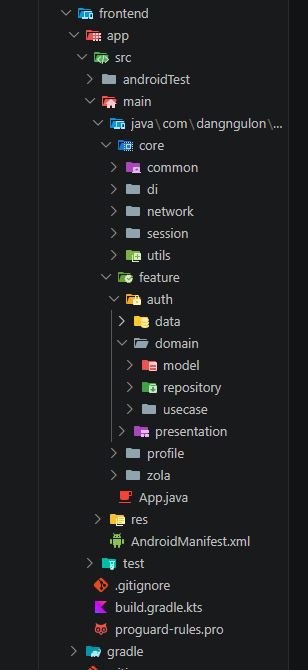
\includegraphics[width=0.9\textwidth]{images/cautrucfejava.png}
    \caption{Cấu trúc frontend Java (mobile)}
\end{figure}

\subsection{Database}

% ========================= LUỒNG HOẠT ĐỘNG =========================
\section{Luồng hoạt động chi tiết của trang web}

\subsection{Luồng đăng ký tài khoản}

\begin{figure}[H]
    \centering
    % Thay bằng ảnh thật của bạn
    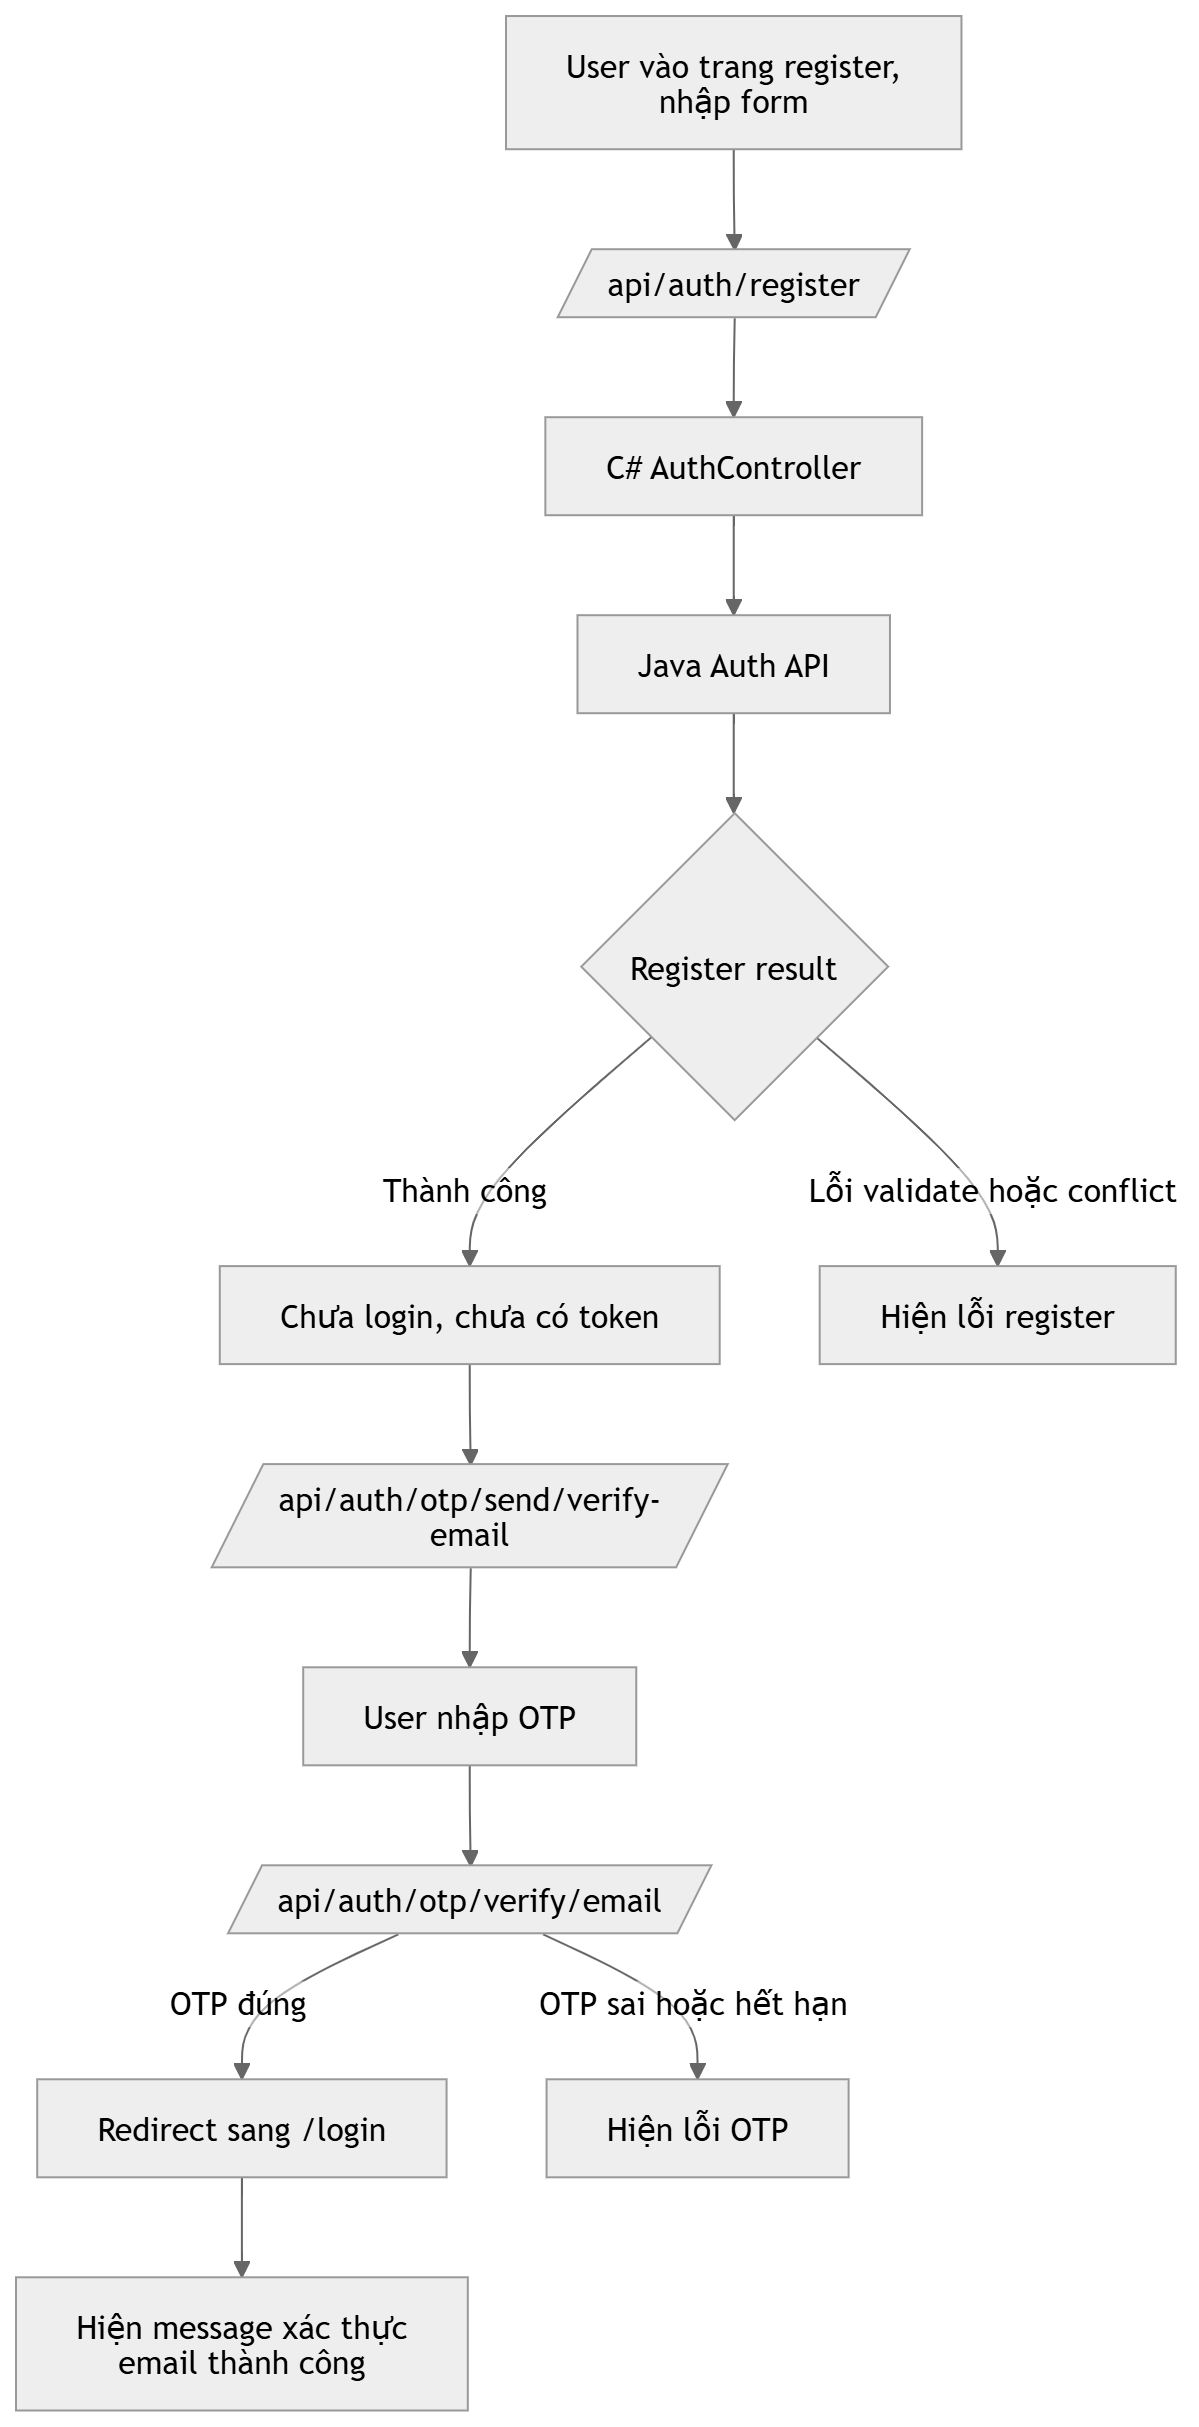
\includegraphics[width=0.6\textwidth]{images/mermaid-diagram (11).png}
    \caption{Luồng đăng ký tài khoản}
\end{figure}

\subsection{Luồng đăng nhập tài khoản}

\begin{figure}[H]
    \centering
    % Thay bằng ảnh thật của bạn
    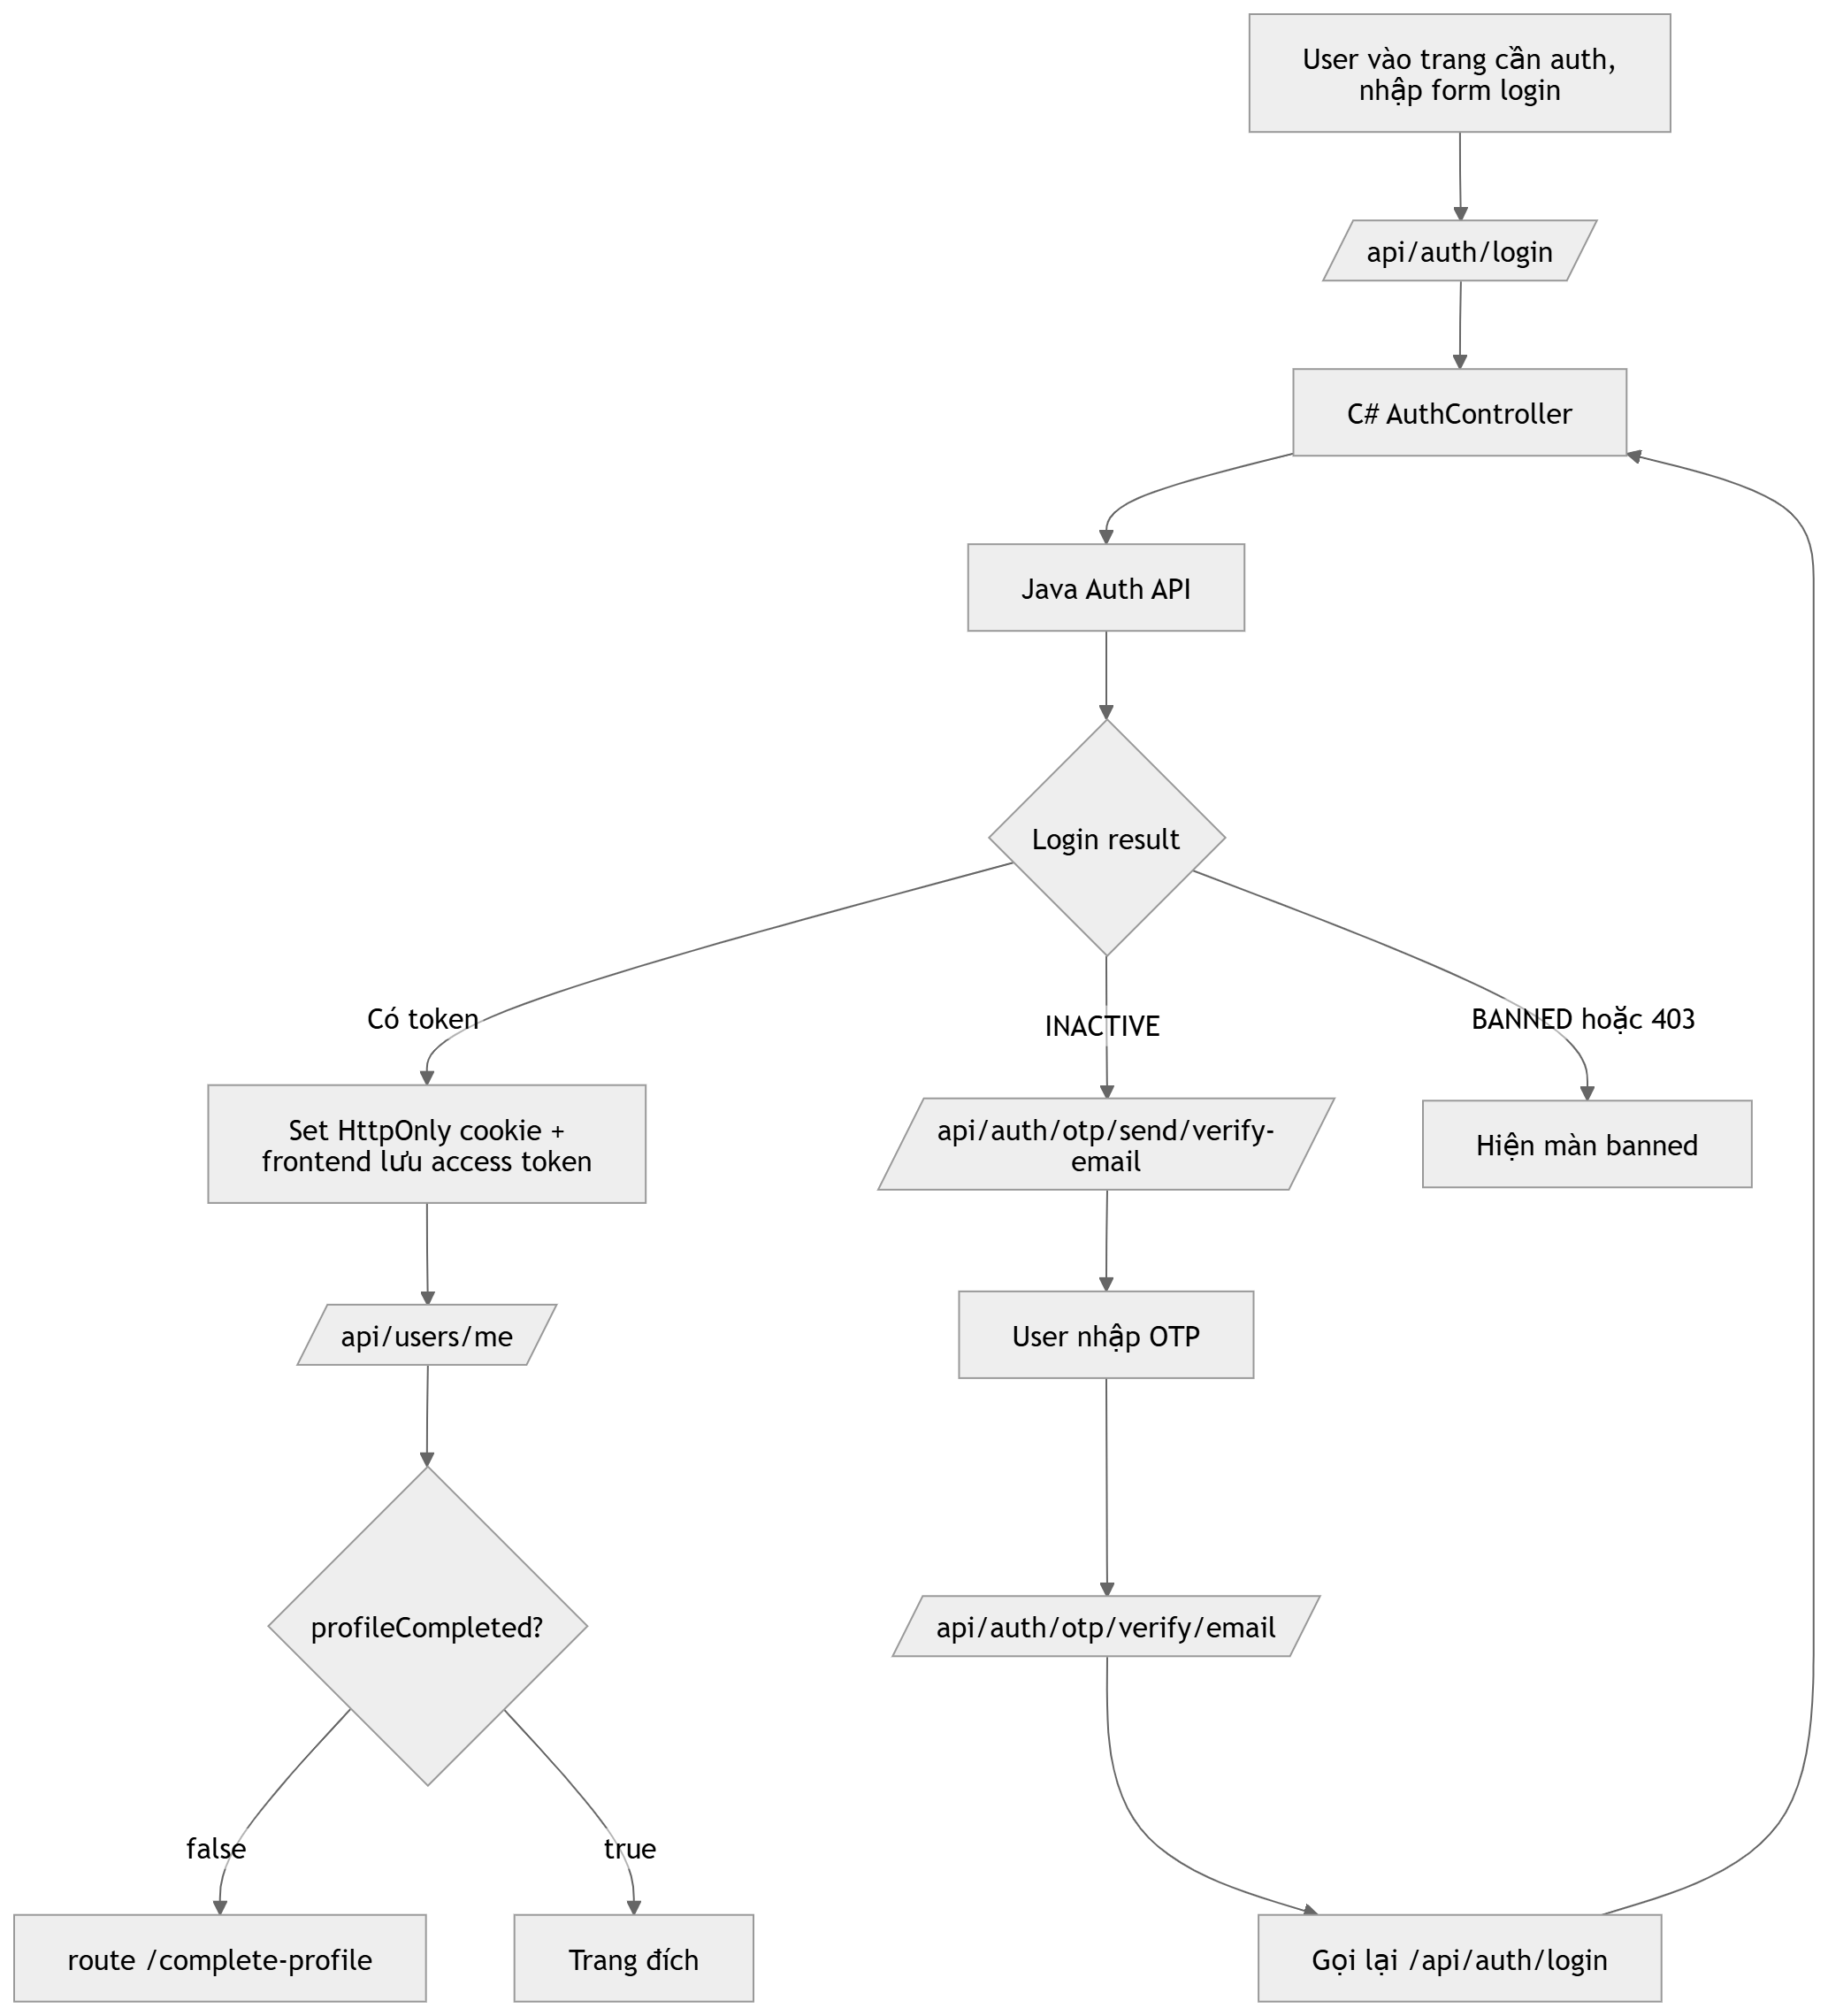
\includegraphics[width=0.9\textwidth]{images/mermaid-diagram (10).png}
    \caption{Luồng đăng nhập tài khoản}
\end{figure}
\begin{figure}[H]
    \centering
    % Thay bằng ảnh thật của bạn
    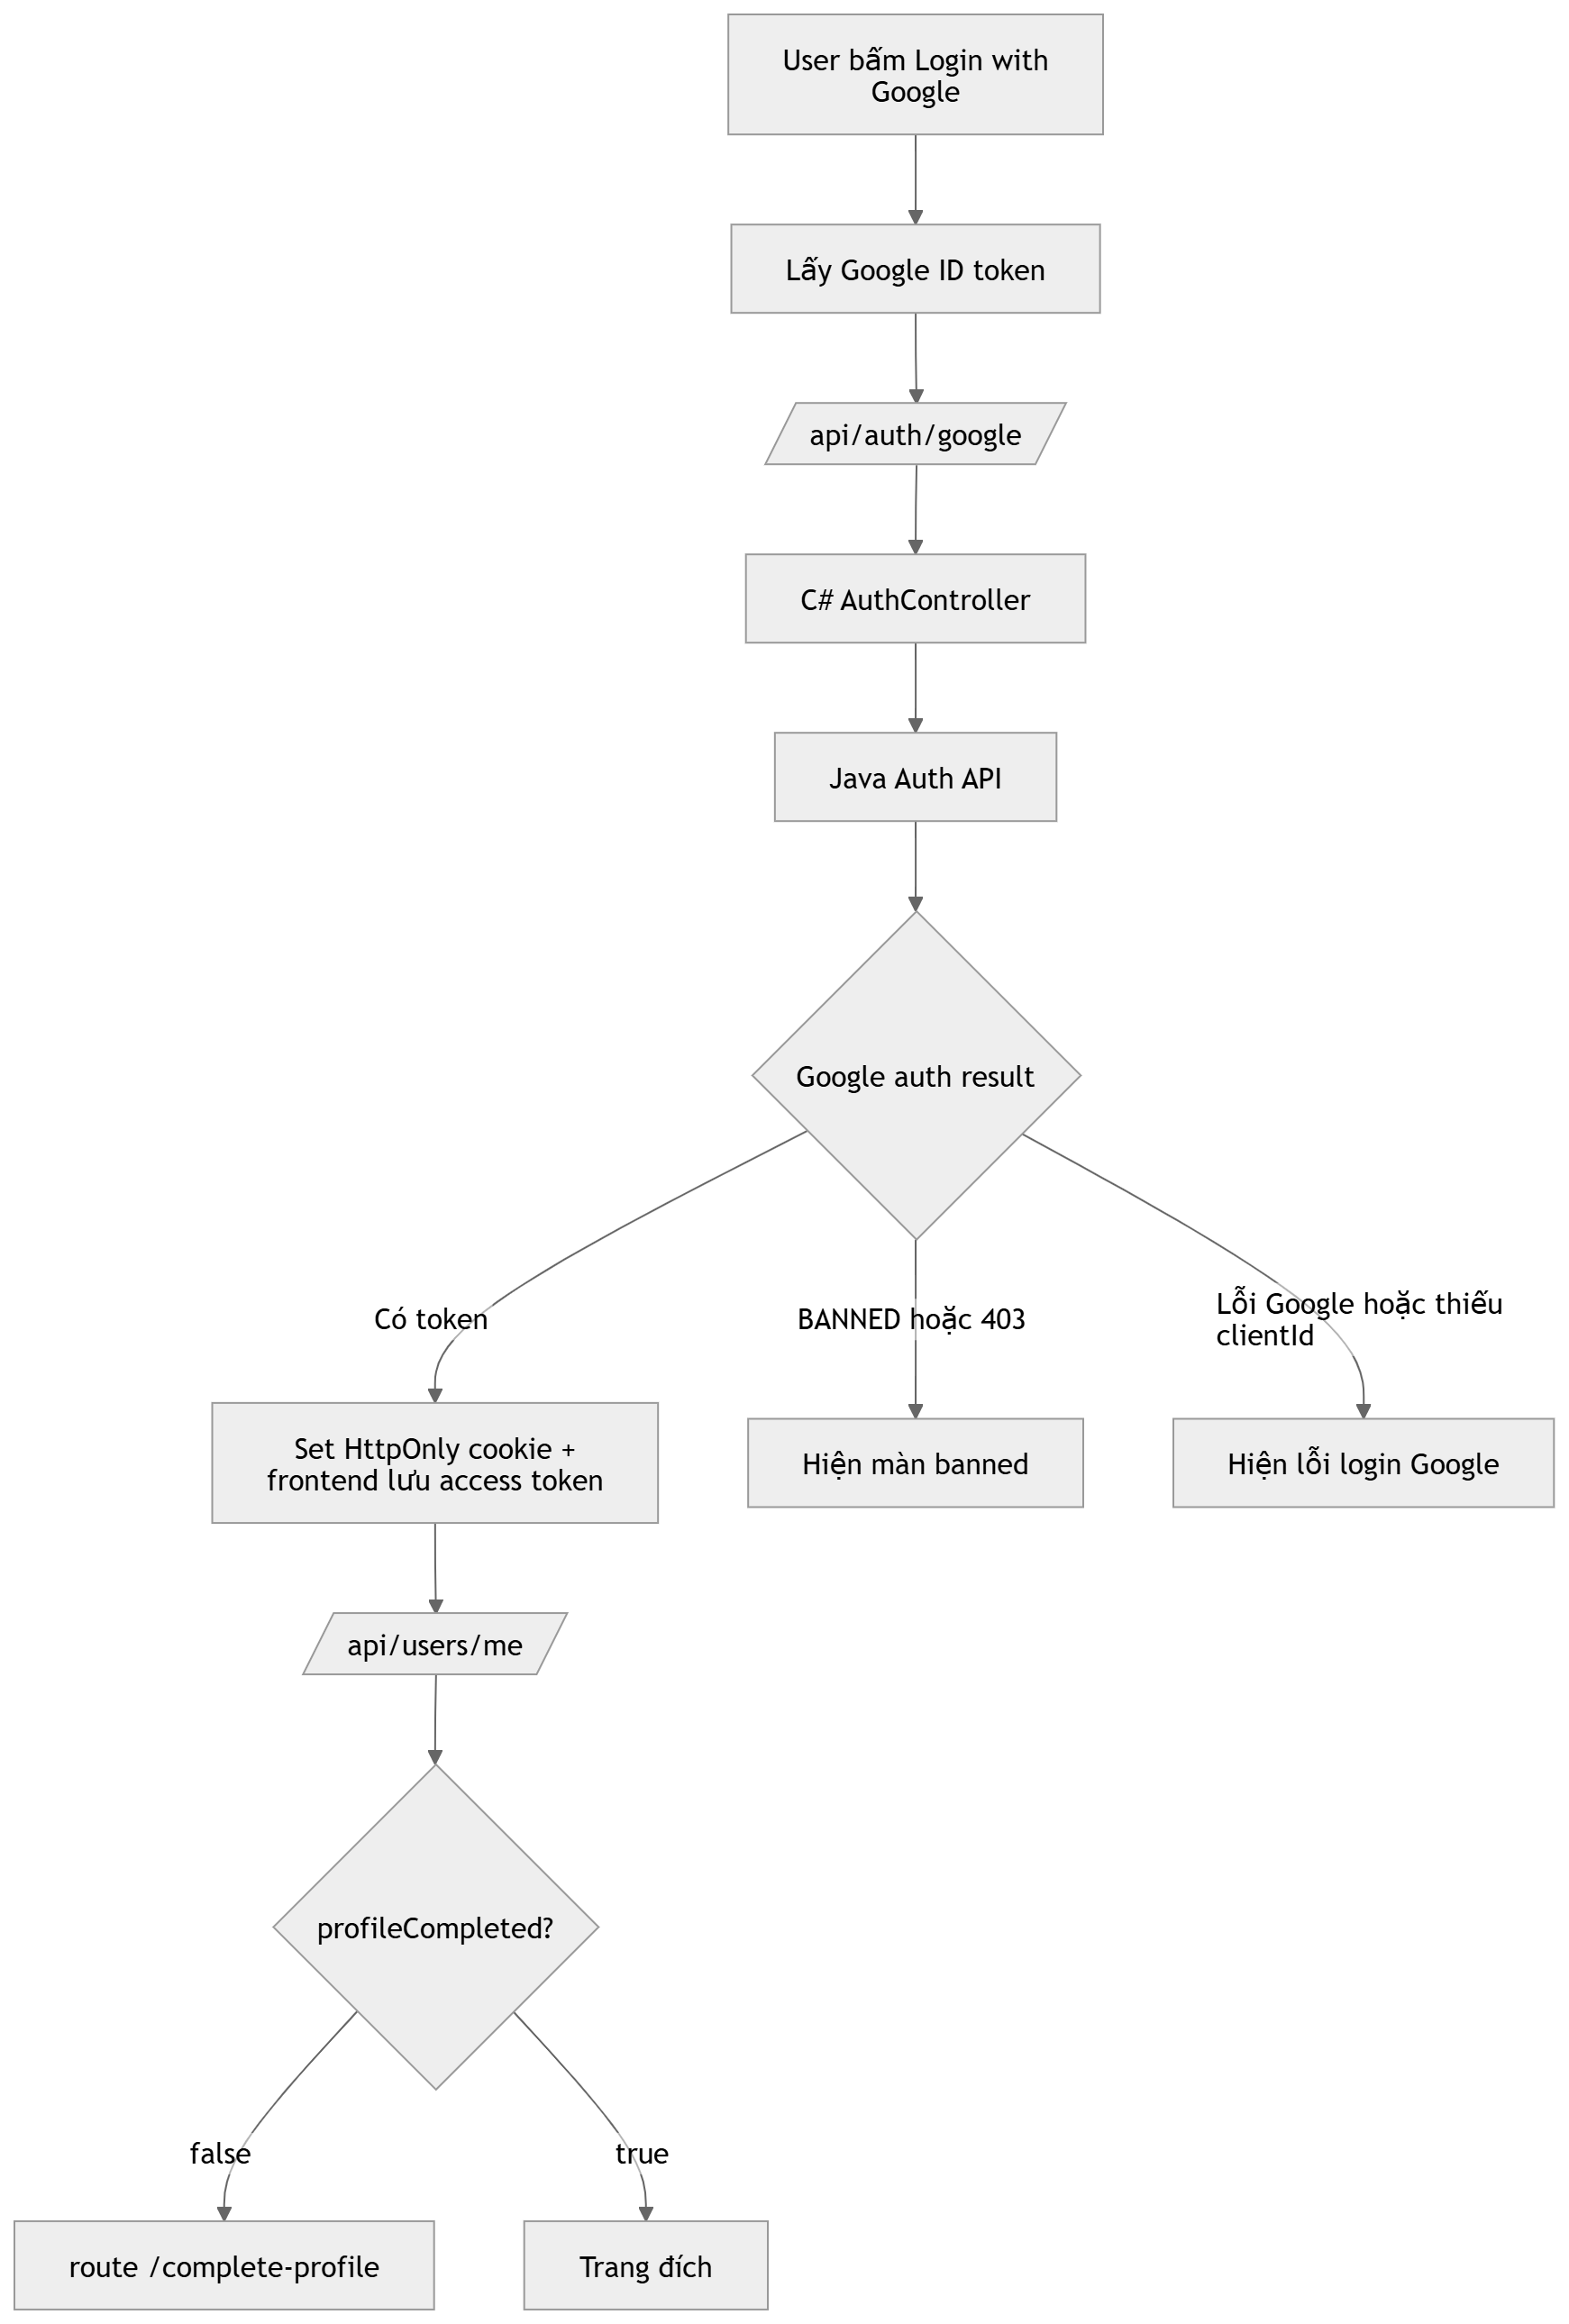
\includegraphics[width=0.8\textwidth]{images/mermaid-diagram (9).png}
    \caption{Luồng đăng nhập tài khoản bằng tài khoản google}
\end{figure}

\subsection{Luồng tải bảng tin (News Feed)}

\begin{figure}[H]
    \centering
    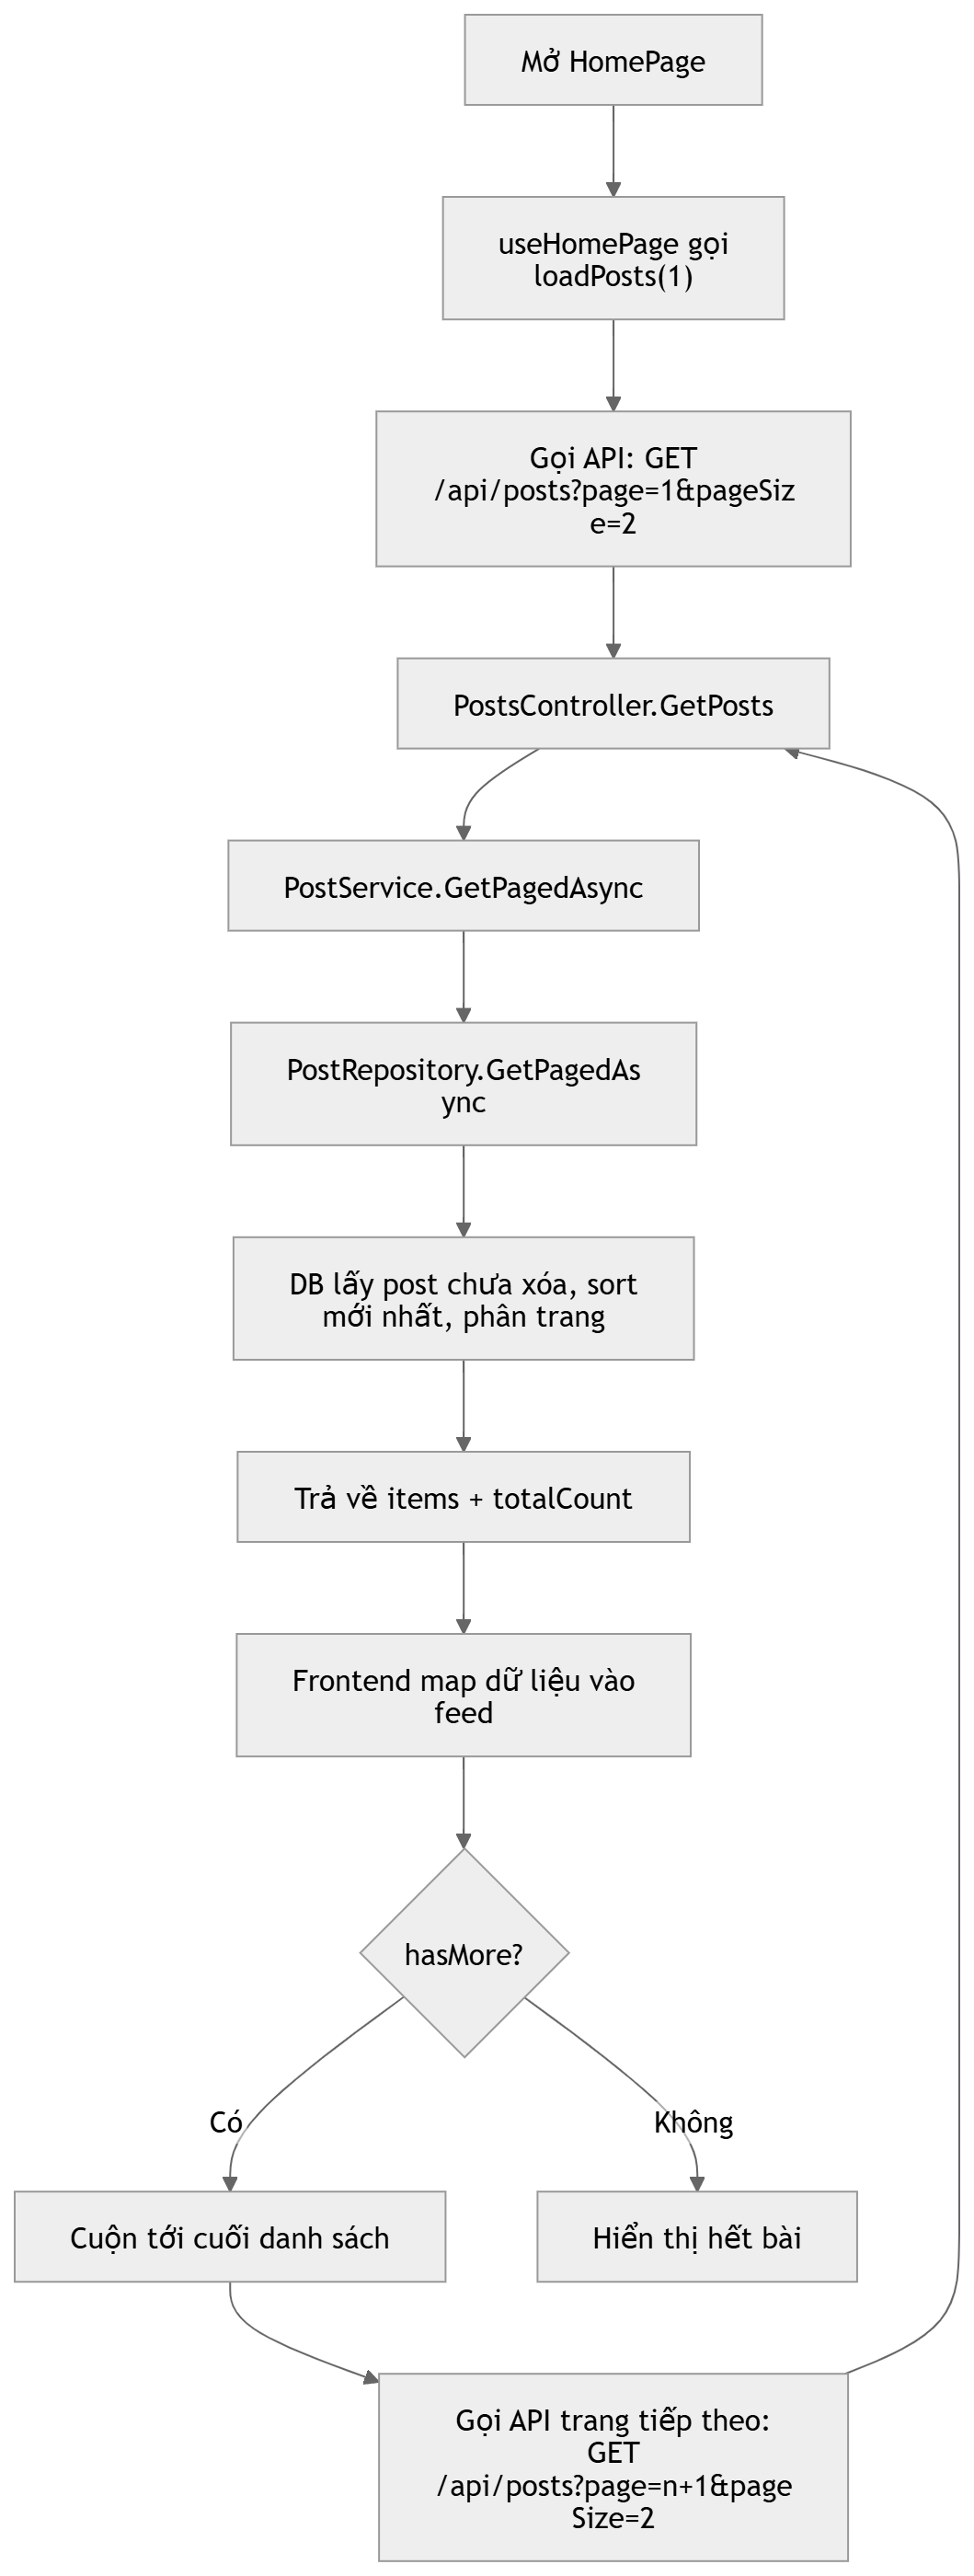
\includegraphics[width=0.5\textwidth]{images/mermaid-diagram (13).png}
    \caption{Luồng tải bảng tin}
    \label{fig:news-feed-flow}
\end{figure}

\subsection{Luồng đăng bài viết mới}
\begin{figure}[H]
    \centering
    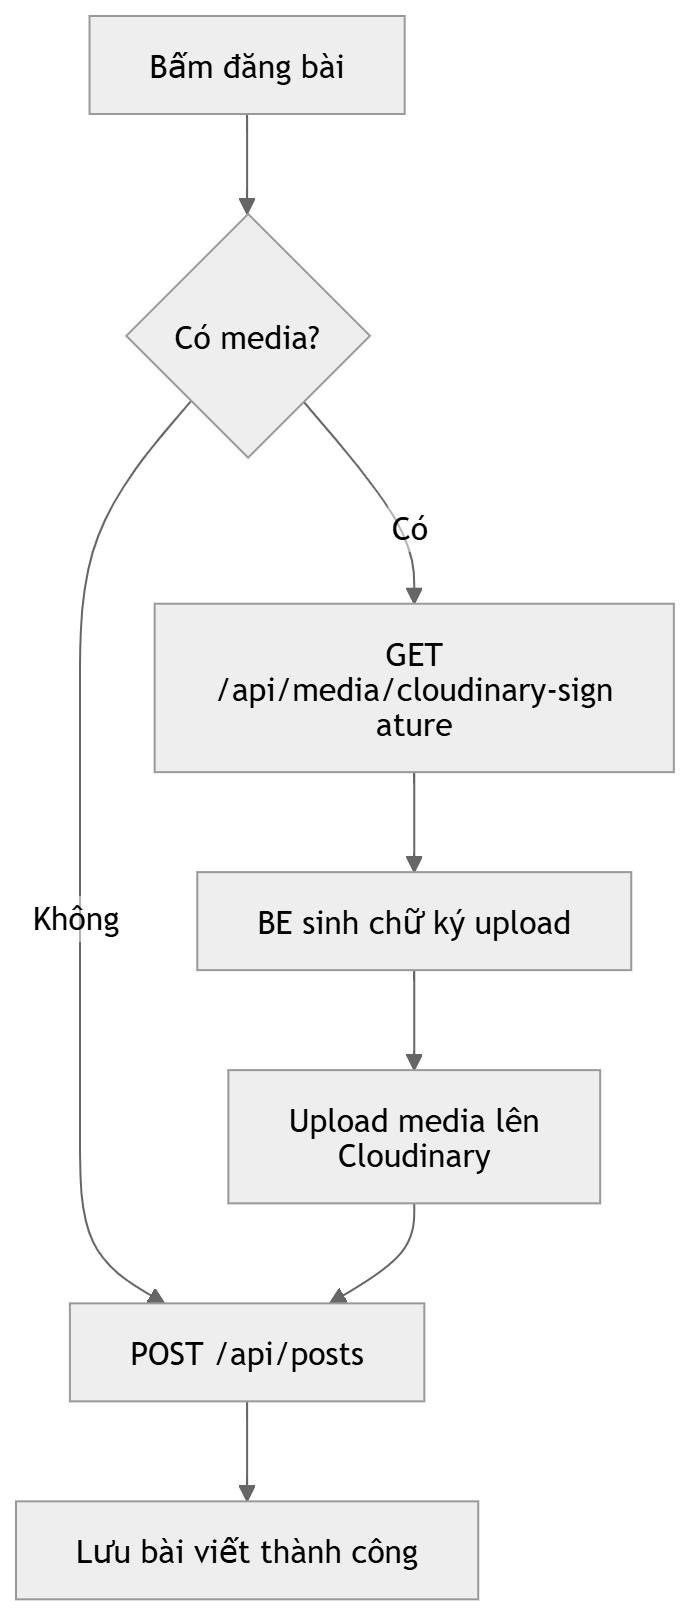
\includegraphics[width=0.6\textwidth]{images/mermaid-diagram (15).png}
    \caption{Luồng đăng post}
    \label{fig:news-feed-flow}
\end{figure}

\subsection{Luồng thích bài viết}
\begin{figure}[H]
    \centering
    % Thay bằng ảnh thật của bạn
    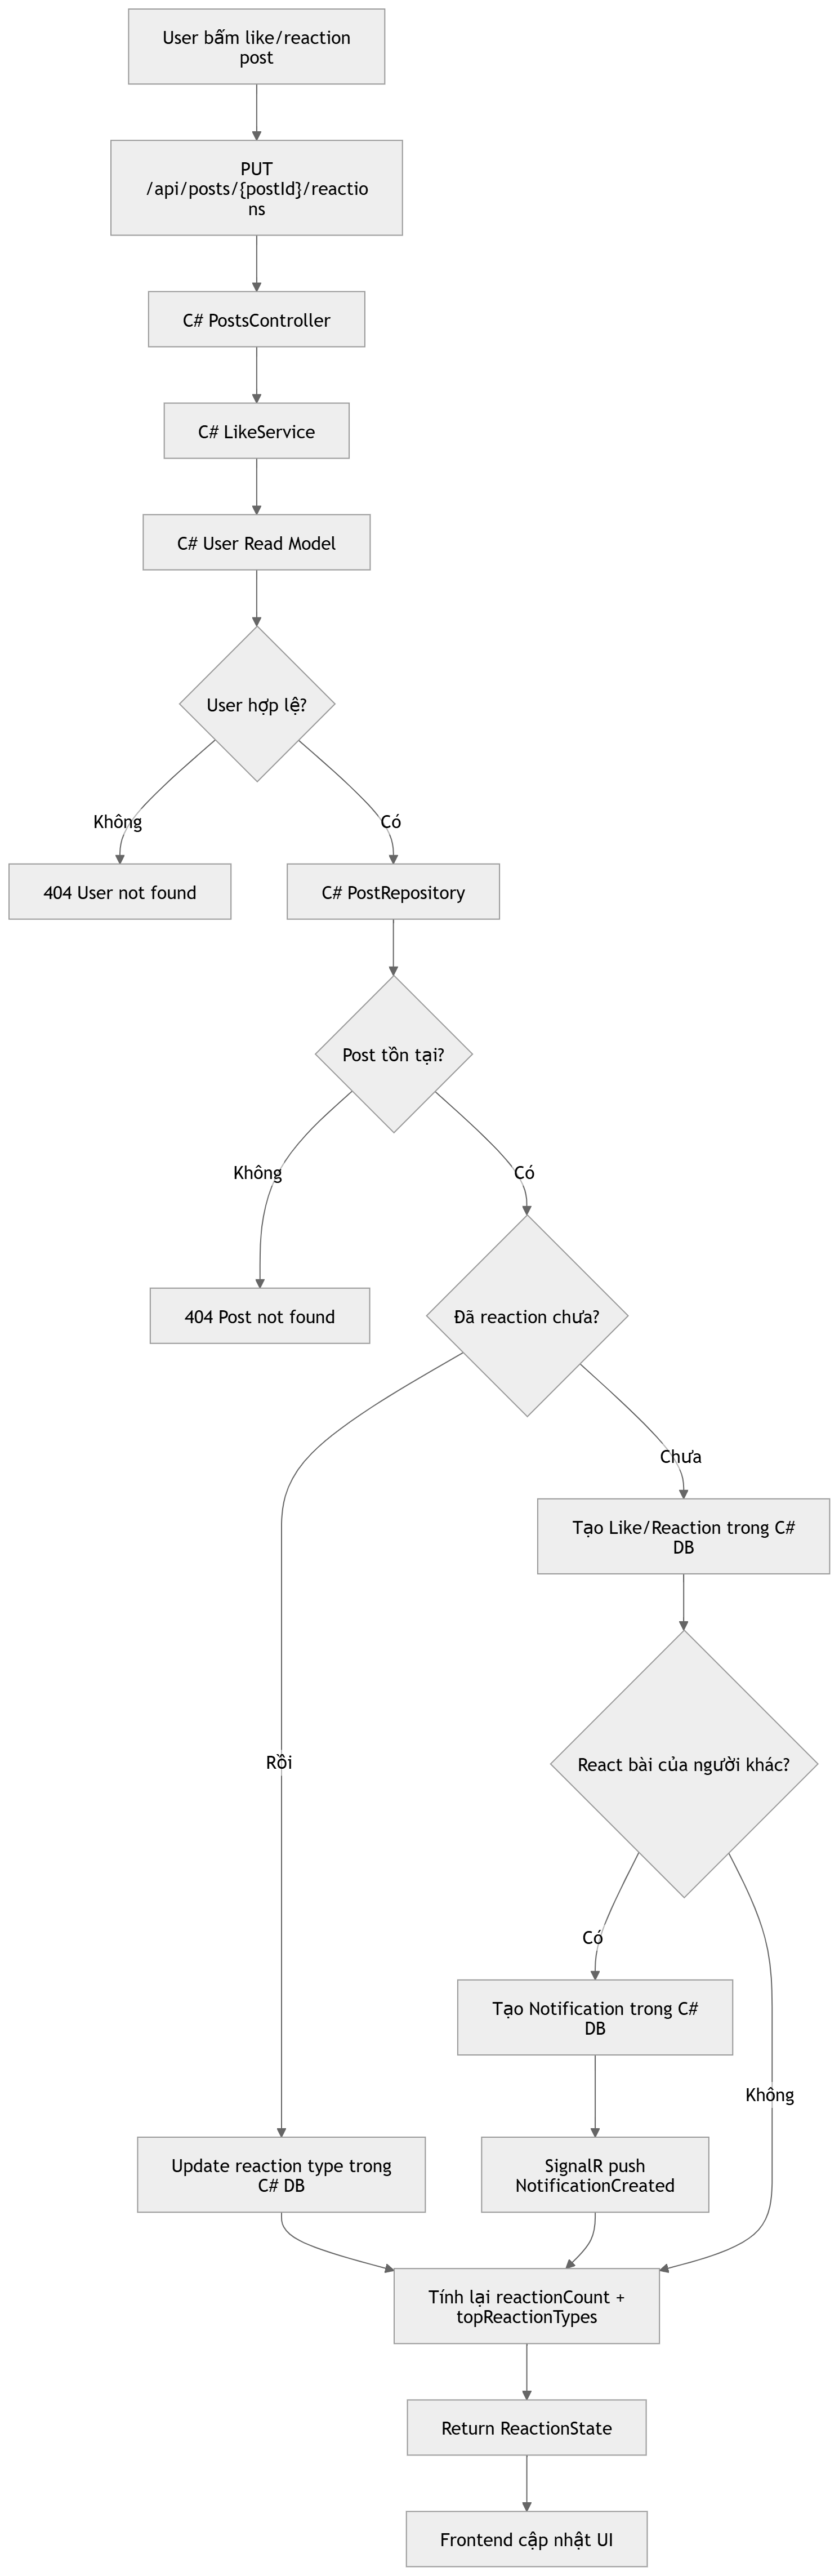
\includegraphics[width=0.4\textwidth]{images/mermaid-diagram (14).png}
    \caption{Luồng lịke}
\end{figure}

\subsection{Luồng bình luận bài viết}
\begin{figure}[H]
    \centering
    % Thay bằng ảnh thật của bạn
    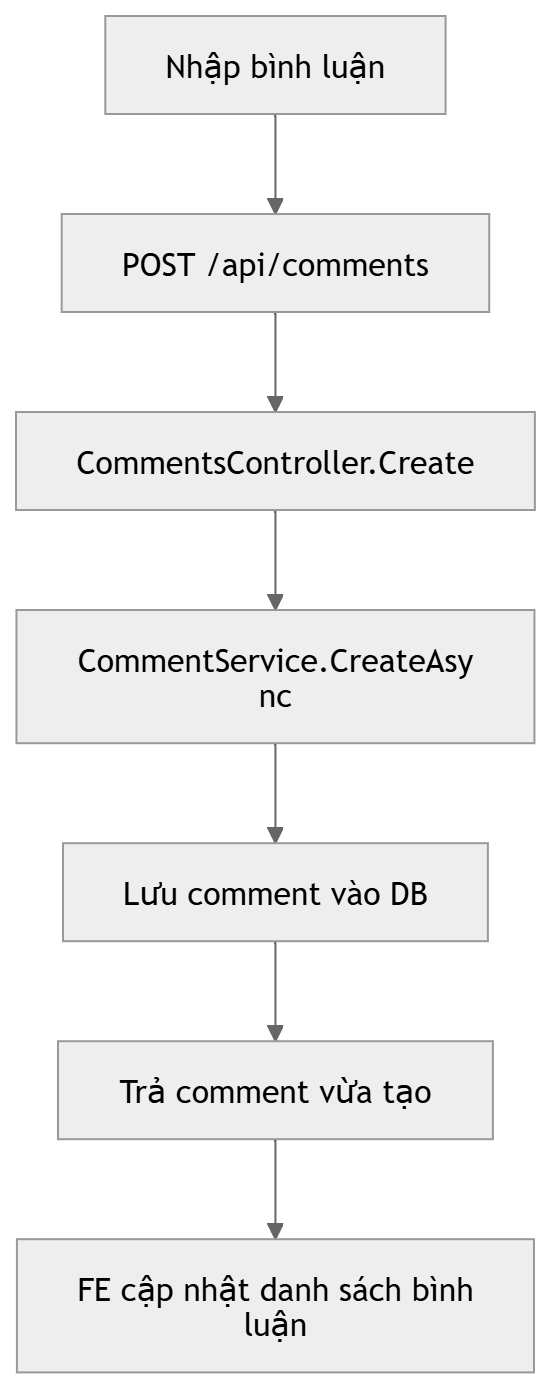
\includegraphics[width=0.5\textwidth]{images/mermaid-diagram (16).png}
    \caption{Luồng comment}
\end{figure}

\subsection{Luồng xem trang cá nhân}
\begin{figure}[H]
    \centering
    % Thay bằng ảnh thật của bạn
    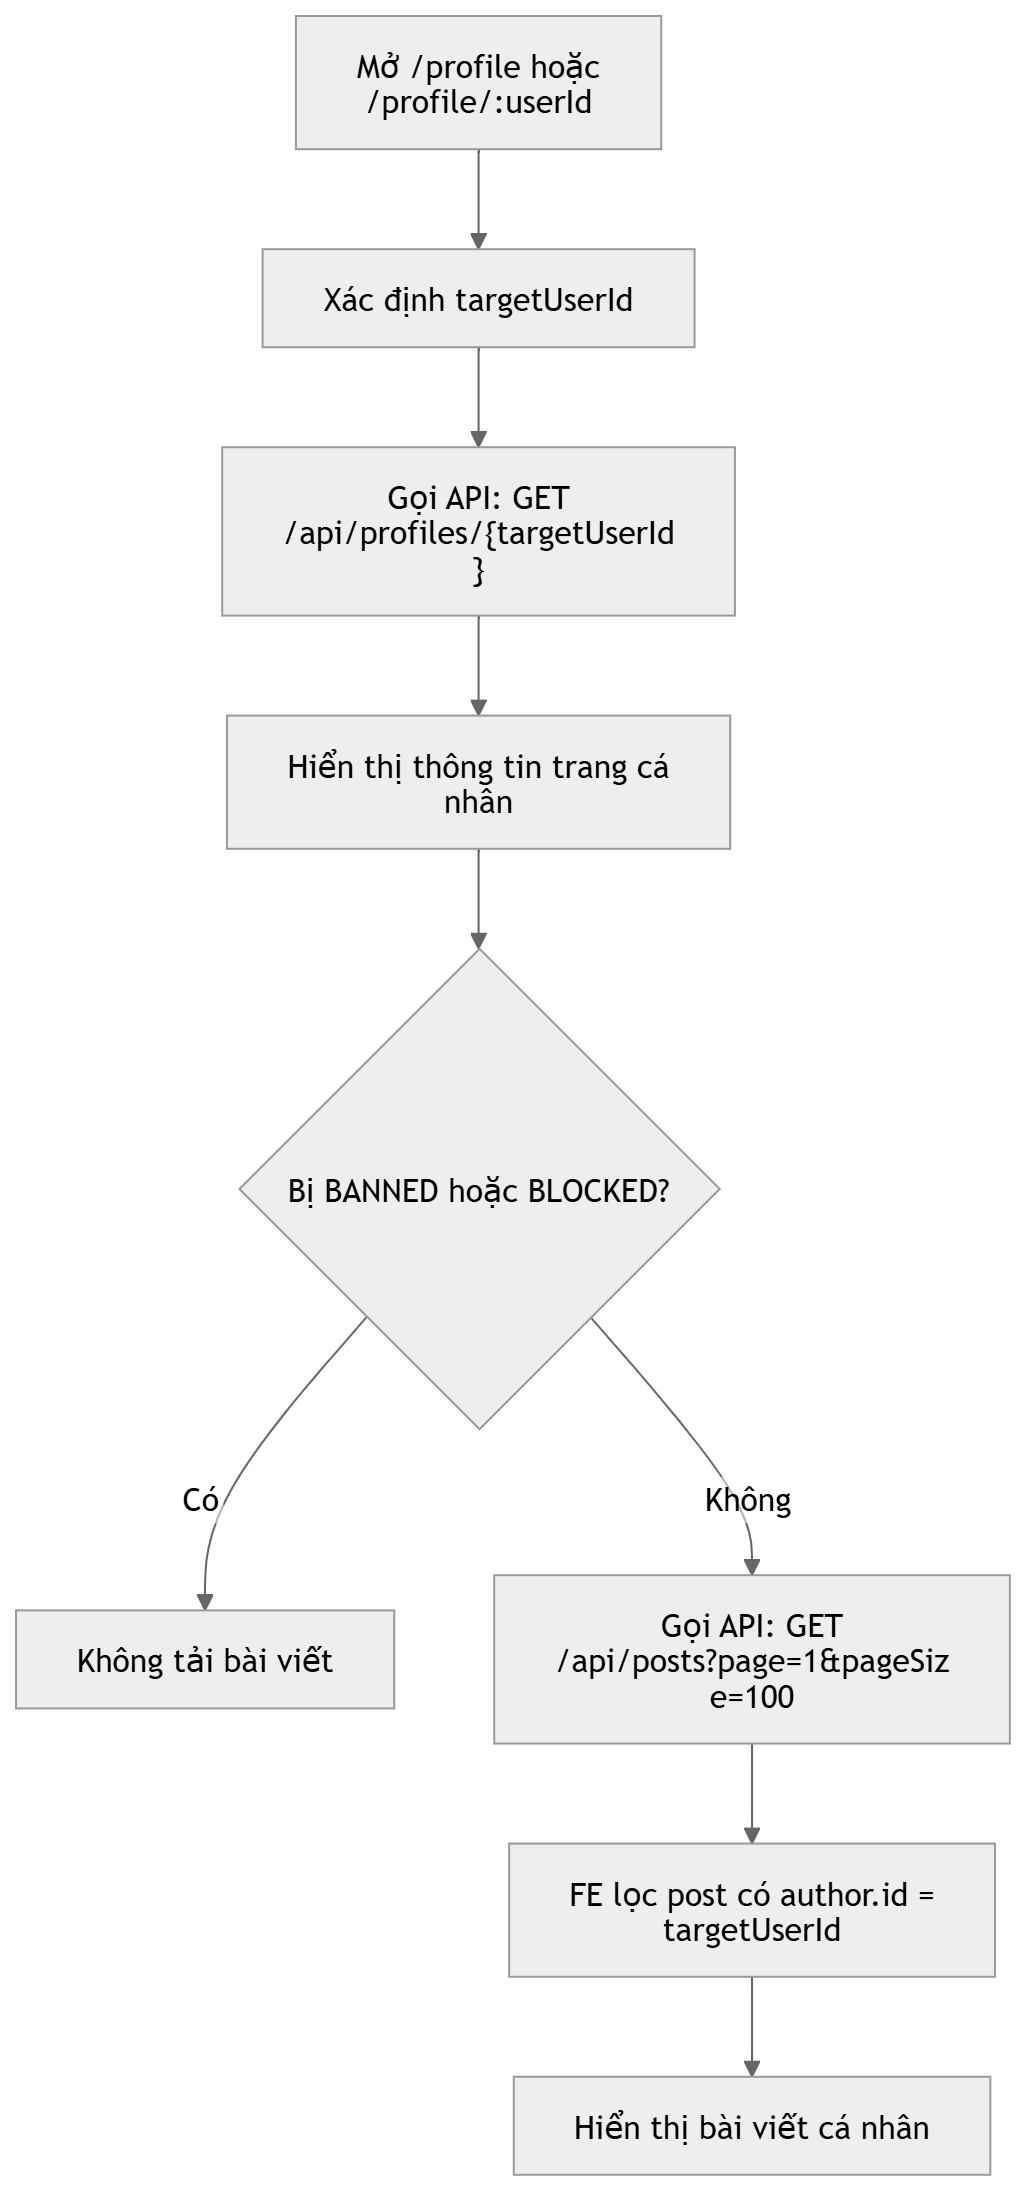
\includegraphics[width=0.6\textwidth]{images/mermaid-diagram (17).png}
    \caption{Luồng xem trang cá nhân}
\end{figure}

\noindent \textbf{Xem thêm các luồng chi tiết:} \url{https://fookbase-flow.pages.dev/}

% ========================= BẢNG API =========================
\section{Danh sách một số API chính}

\small
\begin{longtable}{|>{\raggedright\arraybackslash}p{1.8cm}|>{\raggedright\arraybackslash}p{5.2cm}|>{\raggedright\arraybackslash}p{7cm}|}
\hline
\multicolumn{3}{|c|}{\textbf{C\# API (ASP.NET Core)}} \\
\hline
\textbf{Phương thức} & \textbf{API} & \textbf{Chức năng} \\
\hline
GET & \texttt{/api/posts} & Lấy danh sách bài viết trên bảng tin \\
\hline
POST & \texttt{/api/posts} & Tạo bài viết mới \\
\hline
PUT & \makecell[l]{\texttt{/api/posts/\{postId\}/}\\\texttt{reactions}} & Thả cảm xúc hoặc thay đổi cảm xúc cho bài viết \\
\hline
POST & \texttt{/api/comments} & Tạo bình luận cho bài viết \\
\hline
GET & \makecell[l]{\texttt{/api/profiles/}\\\texttt{\{userId\}}} & Lấy thông tin hồ sơ người dùng \\
\hline
PATCH & \texttt{/api/profiles/me} & Cập nhật hồ sơ cá nhân \\
\hline
GET & \texttt{/api/notifications} & Lấy danh sách thông báo của người dùng \\
\hline
POST & \texttt{/api/stories} & Tạo story mới \\
\hline

\multicolumn{3}{|c|}{\textbf{Java API (Spring Boot)}} \\
\hline
\textbf{Phương thức} & \textbf{API} & \textbf{Chức năng} \\
\hline
POST & \texttt{/api/auth/register} & Đăng ký tài khoản mới \\
\hline
POST & \texttt{/api/auth/login} & Đăng nhập hệ thống \\
\hline
POST & \makecell[l]{\texttt{/api/profiles/me/}\\\texttt{complete-profile}} & Hoàn thiện hồ sơ người dùng sau đăng ký \\
\hline
POST & \texttt{/api/messenger/friendships} & Gửi lời mời kết bạn \\
\hline
GET & \makecell[l]{\texttt{/api/messenger/}\\\texttt{conversations/getByUser}} & Lấy danh sách cuộc trò chuyện của người dùng \\
\hline
POST & \makecell[l]{\texttt{/api/messenger/}\\\texttt{conversations/create}} & Tạo cuộc trò chuyện hoặc nhóm chat mới \\
\hline
GET & \makecell[l]{\texttt{/api/messenger/messages/}\\\texttt{conversation/\{conversationId\}}} & Lấy danh sách tin nhắn của một cuộc trò chuyện \\
\hline
POST & \texttt{/api/messenger/messages/send} & Gửi tin nhắn \\
\hline
\end{longtable}
\normalsize

\noindent \textbf{Xem chi tiết API của Java:} \url{https://fookbase-java-be.onrender.com/swagger-ui/index.html}\\
\textbf{Xem chi tiết API của C\#:} \url{https://fookbase-c-be.onrender.com/swagger/index.html}



% ========================= KẾT QUẢ GIAO DIỆN =========================
\section{Hiển thị kết quả giao diện trang web}

\subsection{Giao diện trang đăng nhập}
\begin{figure}[H]
    \centering
    % Thay bằng ảnh thật của bạn
    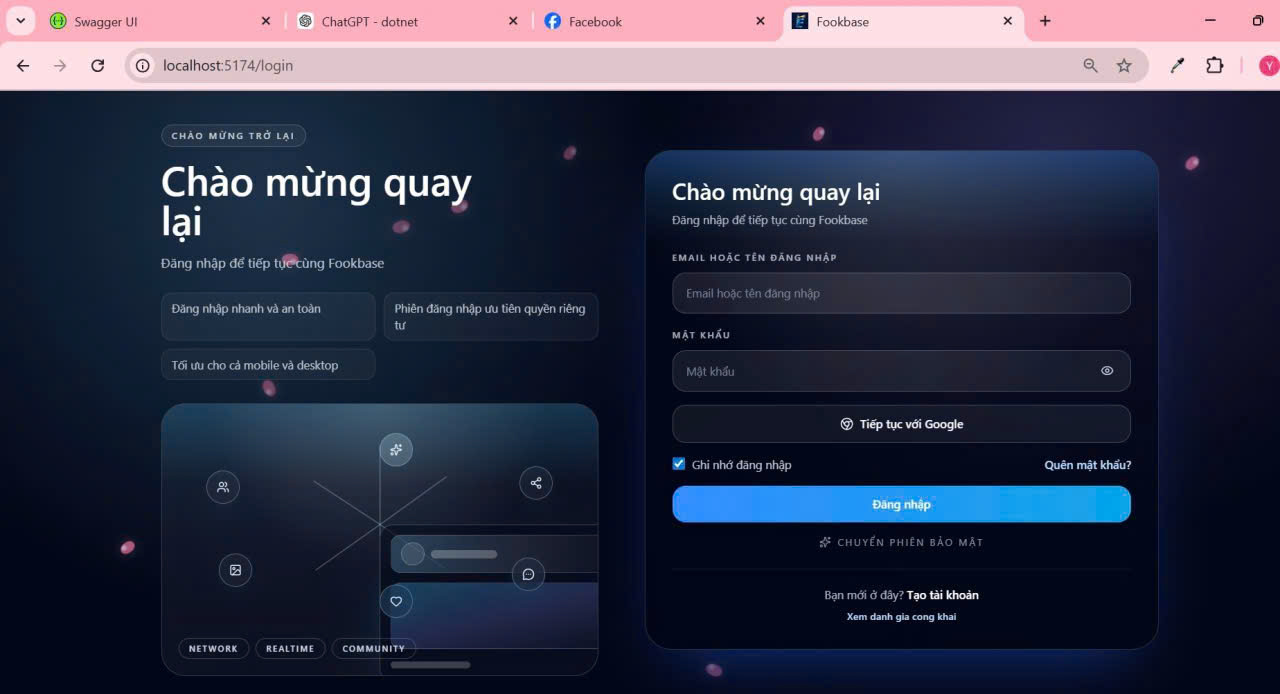
\includegraphics[width=0.85\textwidth]{images/login.jpg}
    \caption{Giao diện trang đăng nhập của Fookbase}
\end{figure}

\subsection{Giao diện trang chủ}
\begin{figure}[H]
    \centering
    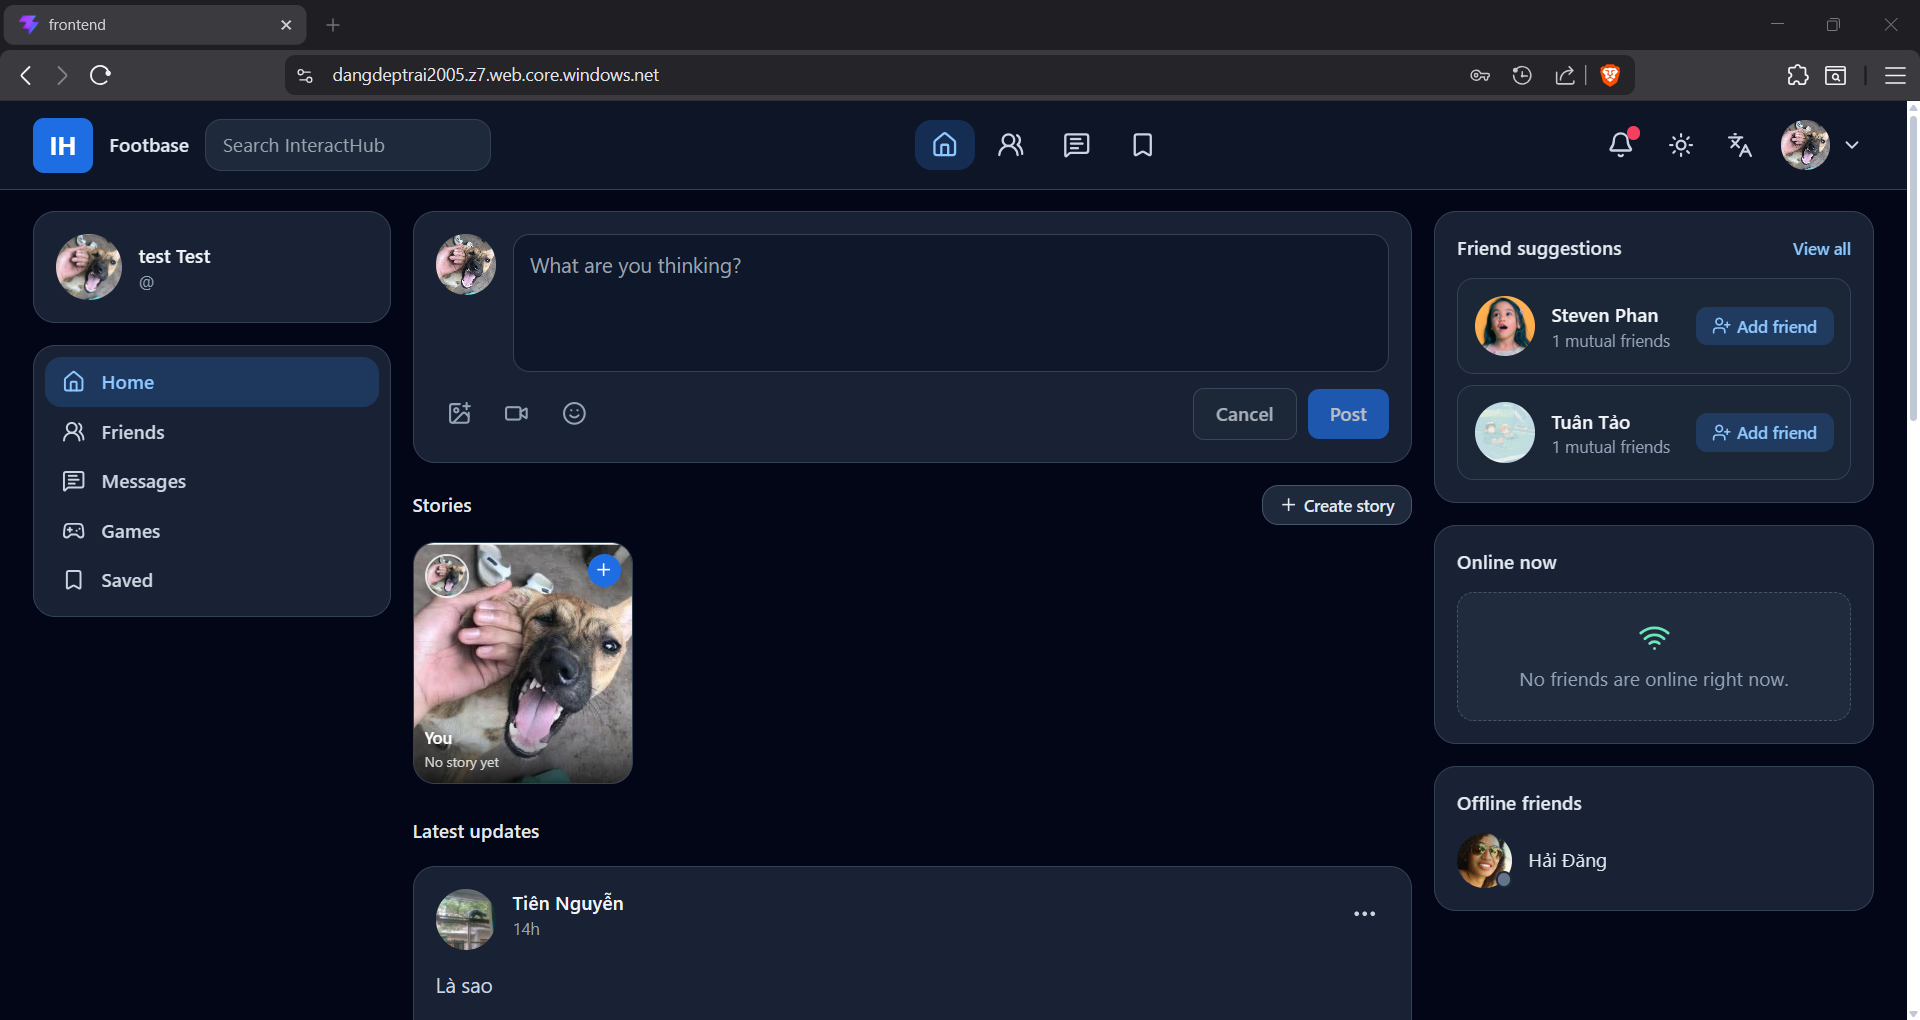
\includegraphics[width=0.85\textwidth]{images/home.png}
    \caption{Giao diện trang chủ hiển thị bảng tin}
\end{figure}

\subsection{Giao diện tạo bài viết}
\begin{figure}[H]
    \centering
    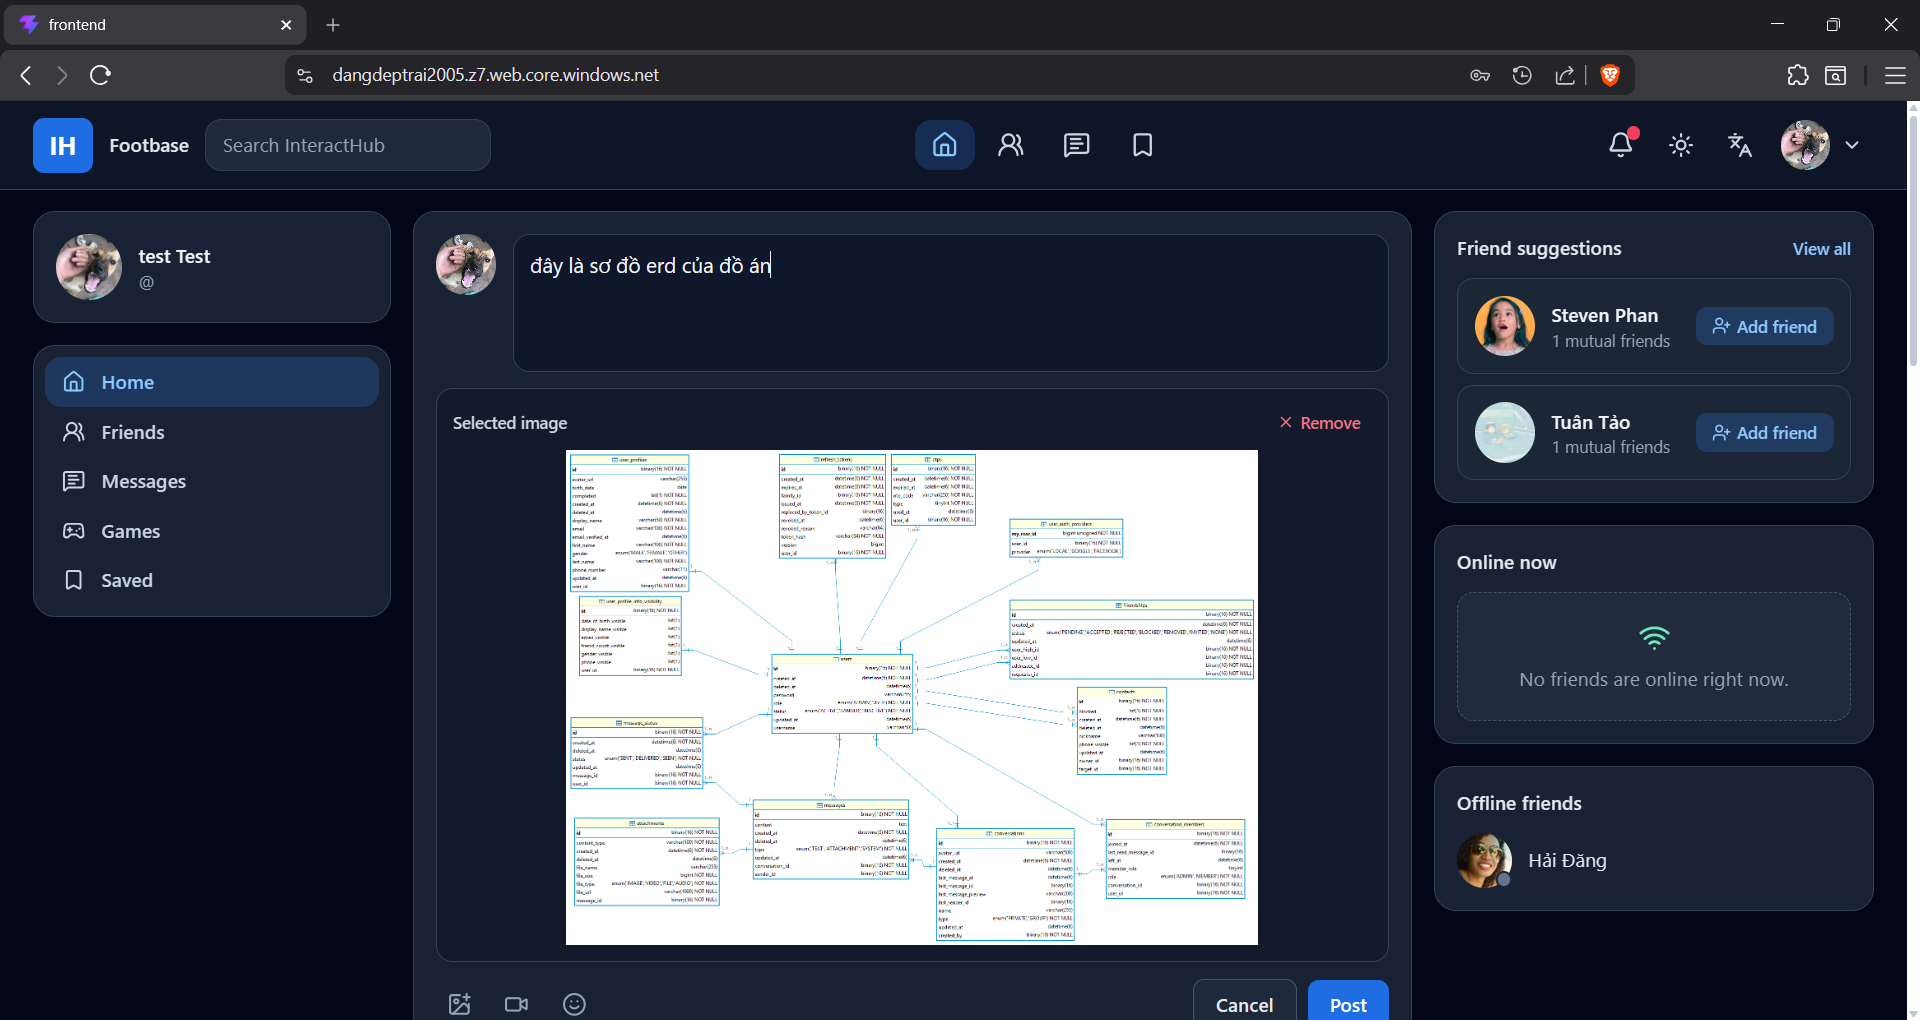
\includegraphics[width=0.85\textwidth]{images/create_post1.png}
    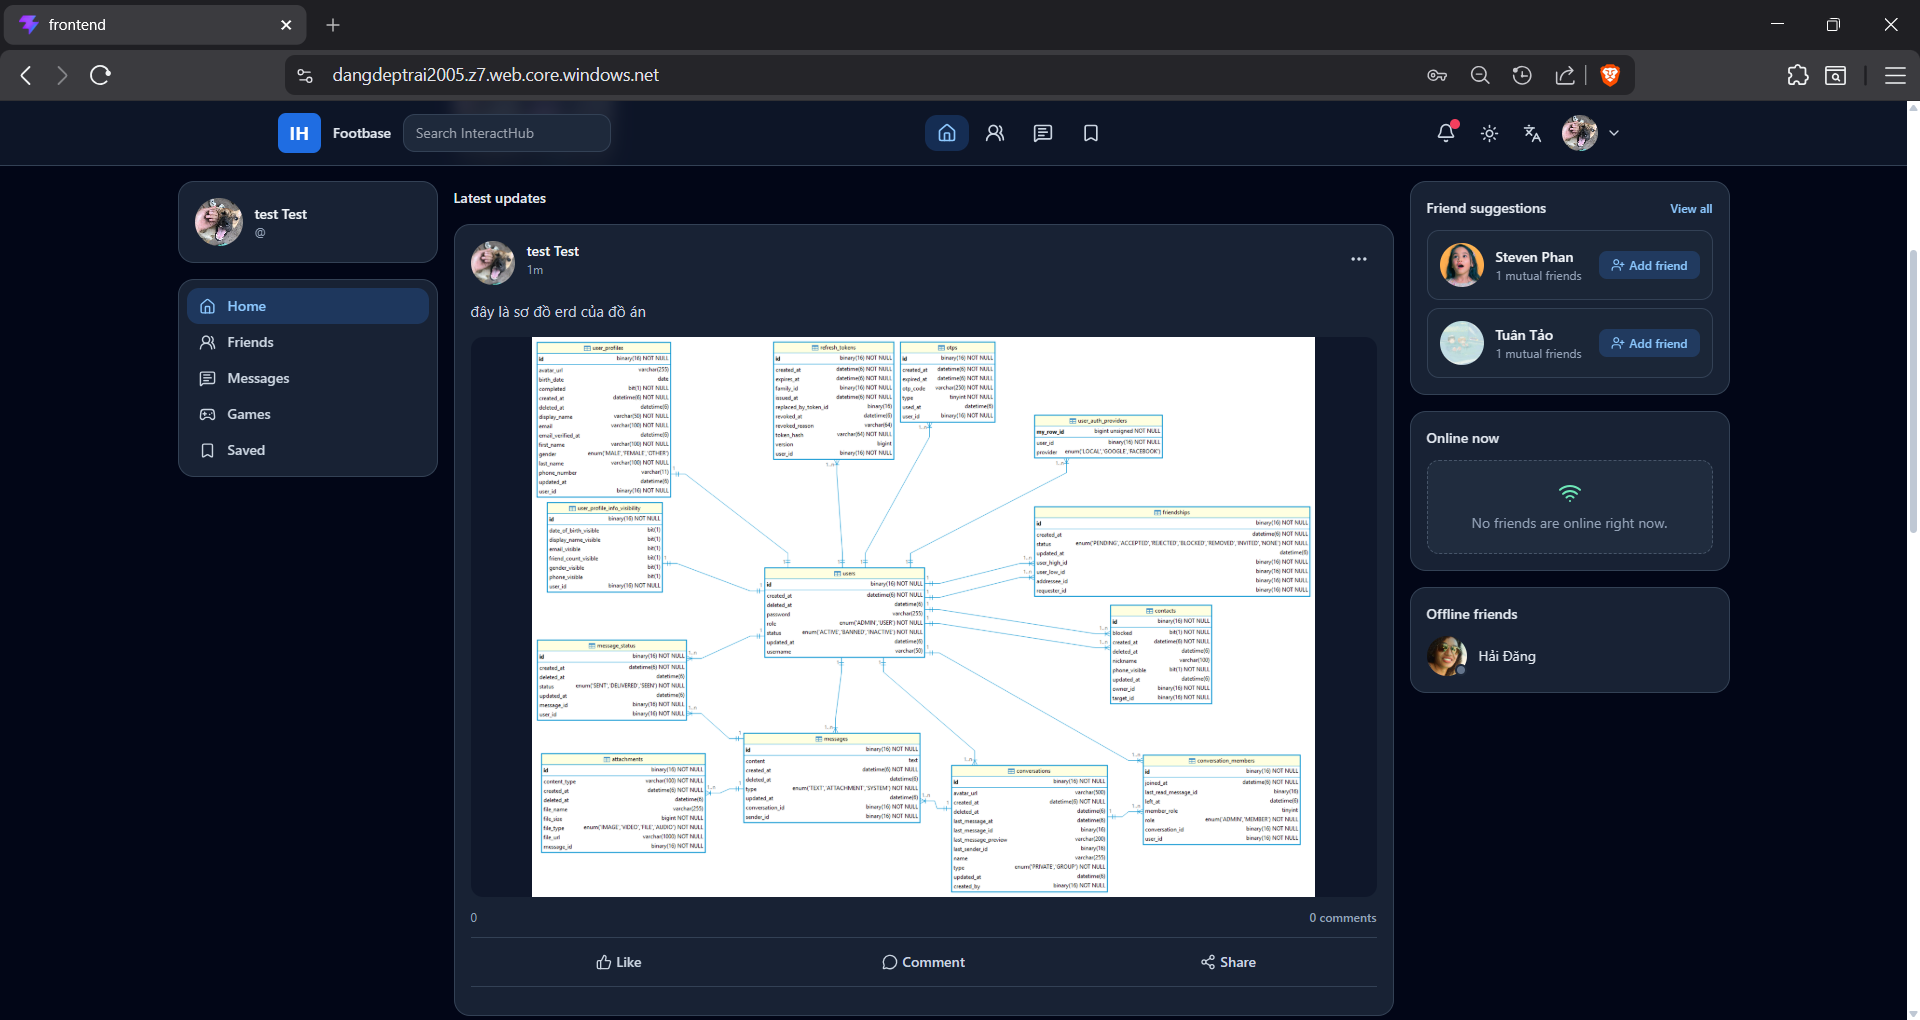
\includegraphics[width=0.85\textwidth]{images/create_post2.png}
    \caption{Chức năng tạo bài viết mới}
\end{figure}

\subsection{Giao diện trang cá nhân}
\begin{figure}[H]
    \centering
    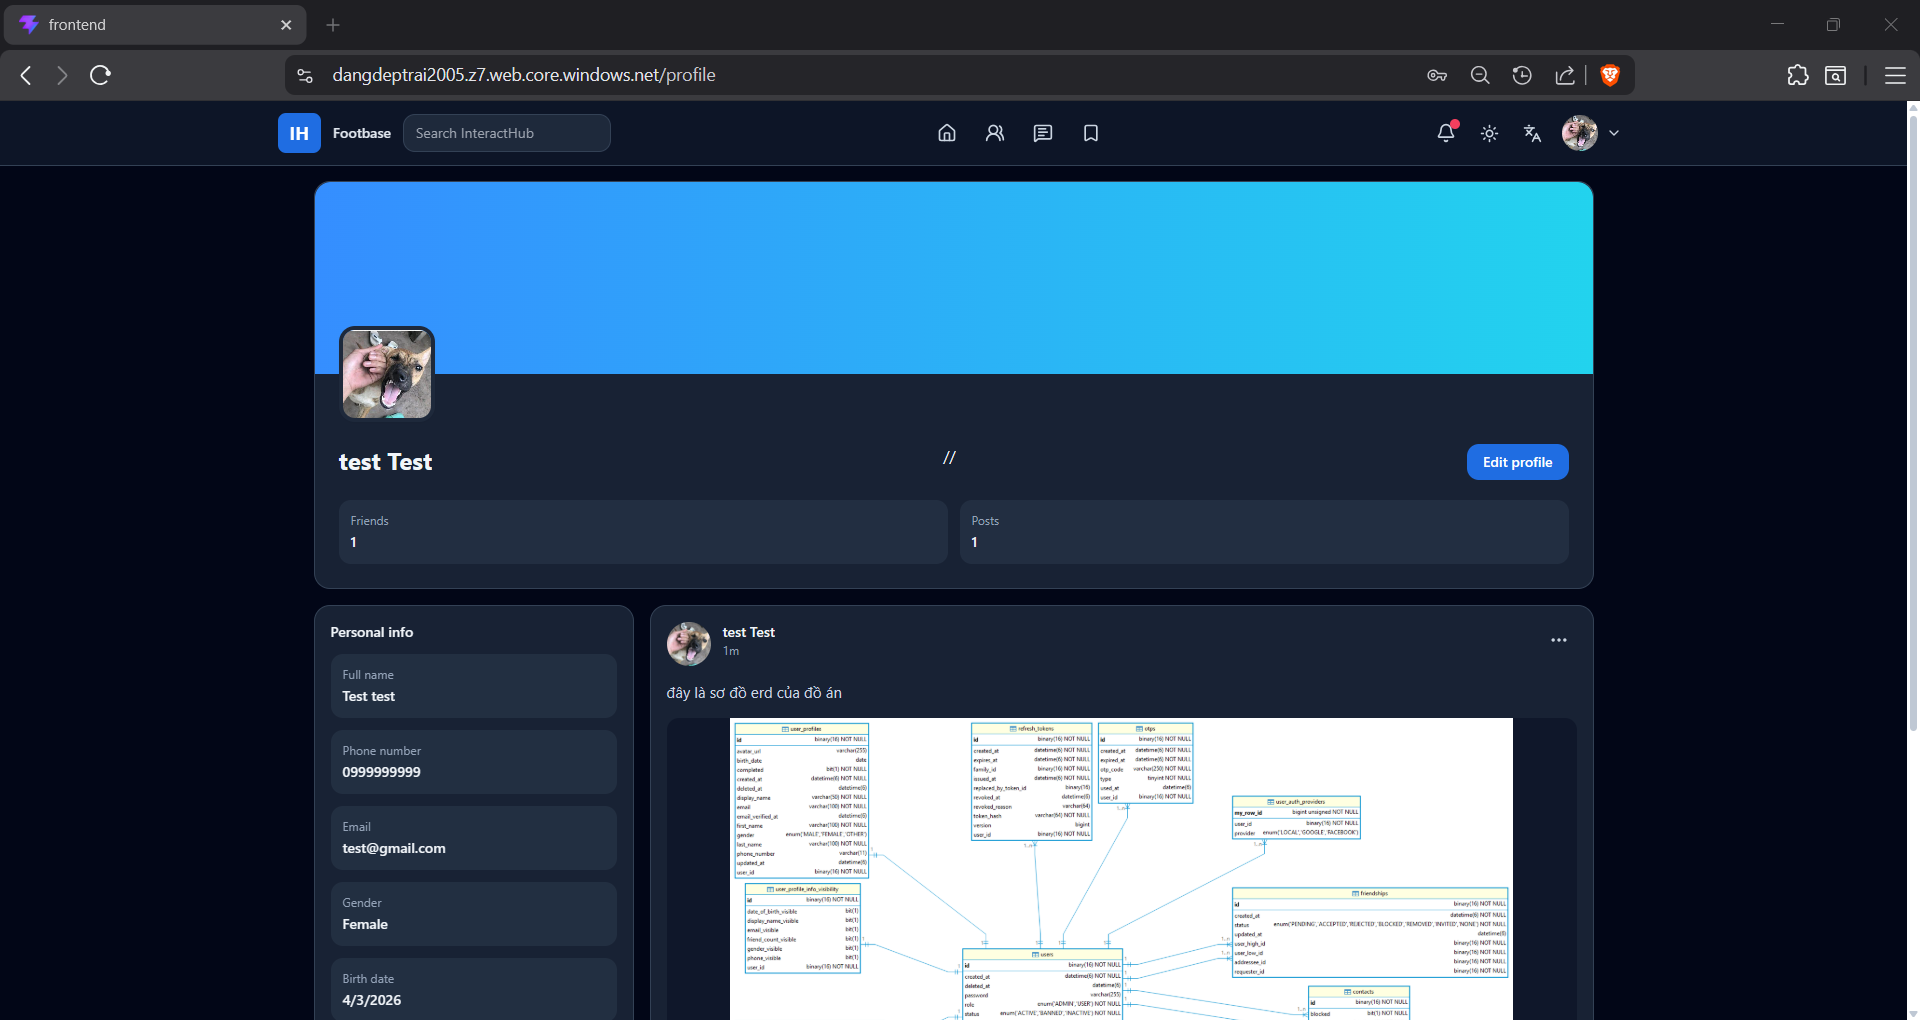
\includegraphics[width=0.85\textwidth]{images/profile.png}
    \caption{Giao diện trang cá nhân người dùng}
\end{figure}

\subsection{Nhận xét kết quả}
Sau quá trình xây dựng và chạy thử, hệ thống Fookbase đã thực hiện được các chức năng chính như đăng nhập, hiển thị bảng tin, tạo bài viết, thích bài viết, bình luận và xem hồ sơ cá nhân. Giao diện có khả năng phản hồi đúng theo dữ liệu nhận từ API, thể hiện được mối liên kết giữa frontend, backend và cơ sở dữ liệu.

% ========================= KIỂM THỬ =========================
\section{Kiểm thử hệ thống}

\subsection{Mục tiêu kiểm thử}
Phần kiểm thử được thực hiện nhằm đảm bảo:
\begin{itemize}
    \item Các API của cả backend Java và backend C\# hoạt động đúng theo yêu cầu nghiệp vụ.
    \item Luồng tích hợp frontend $\rightarrow$ backend $\rightarrow$ cơ sở dữ liệu trả về dữ liệu đúng định dạng.
    \item Các chức năng cốt lõi của mạng xã hội (đăng nhập, bảng tin, đăng bài, tương tác, hồ sơ) hoạt động ổn định.
    \item Hệ thống xử lý đúng các trường hợp lỗi phổ biến (sai thông tin đăng nhập, tham số không hợp lệ, thiếu token).
\end{itemize}

\subsection{Môi trường và phương pháp kiểm thử}
\begin{itemize}
    \item Môi trường deploy: frontend \url{https://fookbase-dang-dep-trai.pages.dev}, C\# API \url{https://fookbase-c-be.onrender.com}, Java API \url{https://fookbase-java-be.onrender.com}.
    \item Kiểm thử tự động backend C\#: sử dụng xUnit + Moq trong project \texttt{backend/fookbase.API.Tests}.
    \item Kiểm thử tự động backend Java: sử dụng JUnit5 + MockMvc trong module \texttt{chat\_app/backend}.
    \item Kiểm thử tích hợp thủ công: gọi API bằng Swagger và kiểm tra phản hồi giao diện trên web.
\end{itemize}

\subsection{Một số test case chức năng}
\begin{longtable}{|p{0.9cm}|p{2.8cm}|p{5cm}|p{5.3cm}|}
\hline
\textbf{STT} & \textbf{Thành phần} & \textbf{Test case} & \textbf{Kết quả mong đợi} \\
\hline
1 & Java API & POST \texttt{/api/auth/login} với username/password hợp lệ & Trả về 200, có \texttt{accessToken}, \texttt{refreshToken}, set cookie refresh token \\
\hline
2 & Java API & POST \texttt{/api/auth/refresh-token} với refresh token hợp lệ & Trả về 200, token mới được cấp lại đúng định dạng \\
\hline
3 & C\# API & GET \texttt{/api/posts} với bearer token hợp lệ & Trả về danh sách bài viết trên bảng tin, dữ liệu phân trang đúng \\
\hline
4 & C\# API & POST \texttt{/api/posts} với nội dung bài viết hợp lệ & Bài viết mới được tạo thành công và hiển thị trên news feed \\
\hline
5 & C\# API & PUT \texttt{/api/posts/\{postId\}/reactions} với loại cảm xúc hợp lệ & Cảm xúc được cập nhật đúng, số liệu tương tác thay đổi tương ứng \\
\hline
6 & C\# API & POST \texttt{/api/comments} với nội dung bình luận hợp lệ & Bình luận được tạo và xuất hiện trong danh sách bình luận bài viết \\
\hline
7 & Frontend + API & Đăng nhập sai mật khẩu trên giao diện web & Giao diện hiển thị lỗi, không tạo phiên đăng nhập \\
\hline
8 & Frontend + API & Đăng nhập thành công rồi tạo bài viết mới & Giao diện cập nhật trạng thái đăng nhập và bài viết hiển thị đúng sau khi submit \\
\hline
\end{longtable}

\subsection{Ví dụ code test backend C\# (xUnit + Moq)}

\begin{mdframed}[backgroundcolor=gray!10]
\begin{lstlisting}[language={[Sharp]C},caption={Ví dụ test AuthController của backend C\#}]
[Fact]
public async Task Login_ReturnsOk_NormalizesToken_AndSetsCookies()
{
    var request = new LoginRequestDto
    {
        Username = "tester",
        Password = "secret"
    };
    var payload = new LoginResponseDto
    {
        Token = " Bearer access-token ",
        RefreshToken = "refresh-token"
    };

    _javaApiServiceMock
        .Setup(service => service.LoginAsync(request, It.IsAny<CancellationToken>()))
        .ReturnsAsync(JavaApiCallResult<LoginResponseDto>.Success(payload, StatusCodes.Status200OK));

    var httpContext = new DefaultHttpContext();
    var controller = CreateController(httpContext);

    var result = await controller.Login(request, CancellationToken.None);

    var objectResult = Assert.IsType<ObjectResult>(result.Result);
    Assert.Equal(StatusCodes.Status200OK, objectResult.StatusCode);

    _authCookieServiceMock.Verify(
        service => service.SetLoginCookies(httpContext, "access-token", "refresh-token"),
        Times.Once);
}
\end{lstlisting}
\end{mdframed}

\subsection{Ví dụ code test backend Java (JUnit5 + MockMvc)}

\begin{mdframed}[backgroundcolor=gray!10]
\begin{lstlisting}[language=Java,caption={Ví dụ test API đăng nhập của backend Java}]
@Test
void login_shouldReturnTokenAndSetRefreshCookie() throws Exception {
    LoginResponse loginResponse = LoginResponse.builder()
            .token("access-token")
            .accessToken("access-token")
            .refreshToken("refresh-token")
            .tokenType("Bearer")
            .build();

    when(authService.login(any(LoginRequest.class))).thenReturn(loginResponse);
    when(authService.getRefreshTokenExpirationSeconds()).thenReturn(1209600L);

    mockMvc.perform(post("/api/auth/login")
                    .contentType(MediaType.APPLICATION_JSON)
                    .content("""
                            {"username":"alice","password":"Secret123"}
                            """))
            .andExpect(status().isOk())
            .andExpect(jsonPath("$.accessToken").value("access-token"))
            .andExpect(jsonPath("$.refreshToken").value("refresh-token"));
}
\end{lstlisting}
\end{mdframed}

\subsection{Kết quả chạy test tự động}
\begin{itemize}
    \item Backend C\#: chạy lệnh \texttt{dotnet test backend/fookbase.slnx -c Release}, kết quả \textbf{Passed 33/33}, \textbf{Failed 0}, \textbf{Skipped 0}.
    \item Backend Java: chạy lệnh \texttt{mvn -B test} tại \texttt{chat\_app/backend}, kết quả \textbf{Tests run 16}, \textbf{Failures 0}, \textbf{Errors 0}, \textbf{Skipped 1}.
    \item Frontend web: kiểm thử tích hợp theo kịch bản đăng nhập, tải bảng tin, tạo bài viết, bình luận và xem hồ sơ trên môi trường deploy.
\end{itemize}

\subsection{Hình ảnh minh chứng kiểm thử}

\begin{figure}[H]
    \centering
    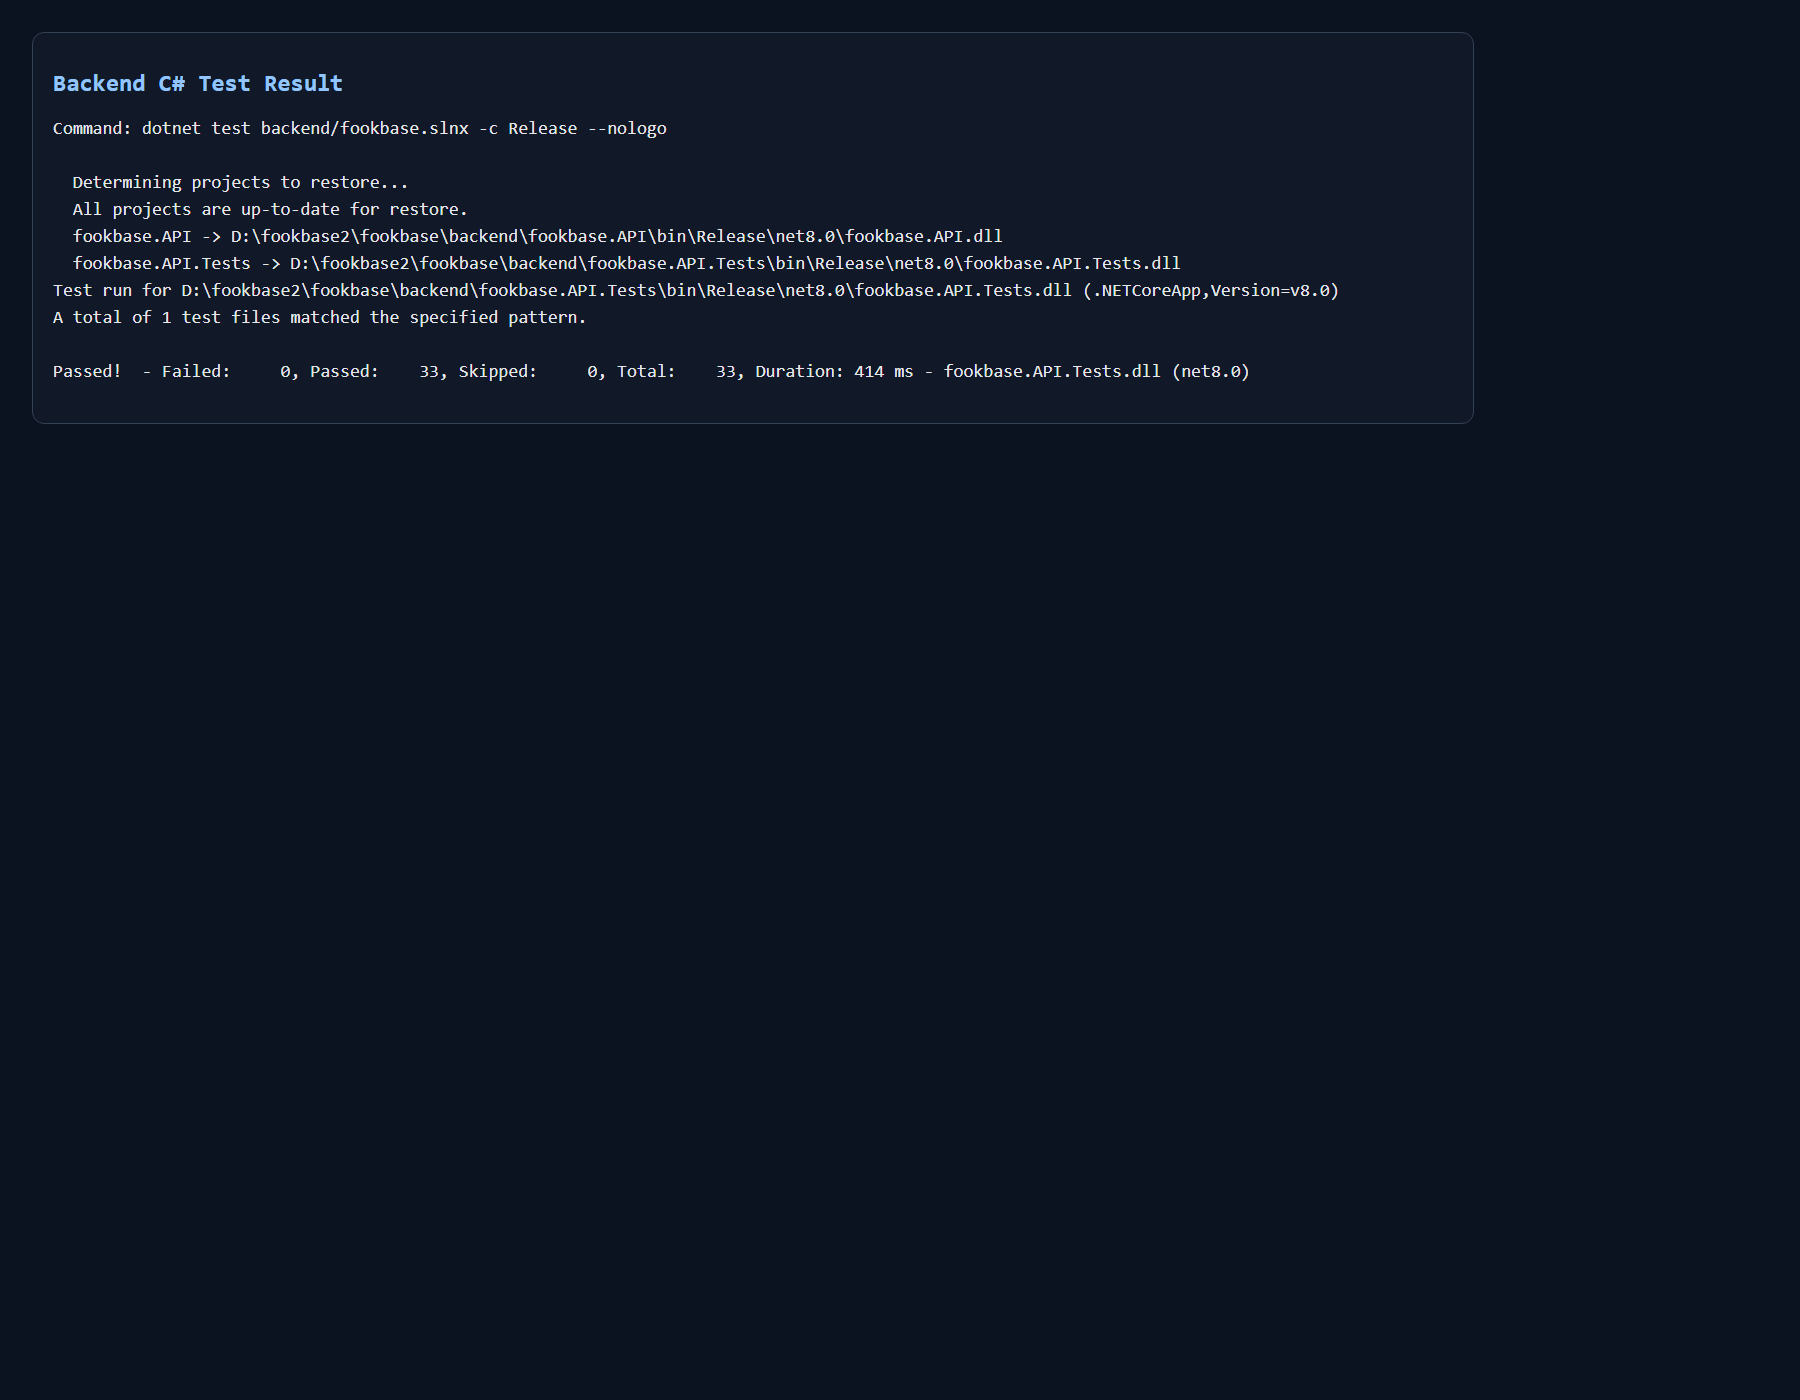
\includegraphics[width=0.95\textwidth]{images/test-shots/test-result-csharp.png}
    \caption{Kết quả chạy test tự động backend C\#}
\end{figure}

\begin{figure}[H]
    \centering
    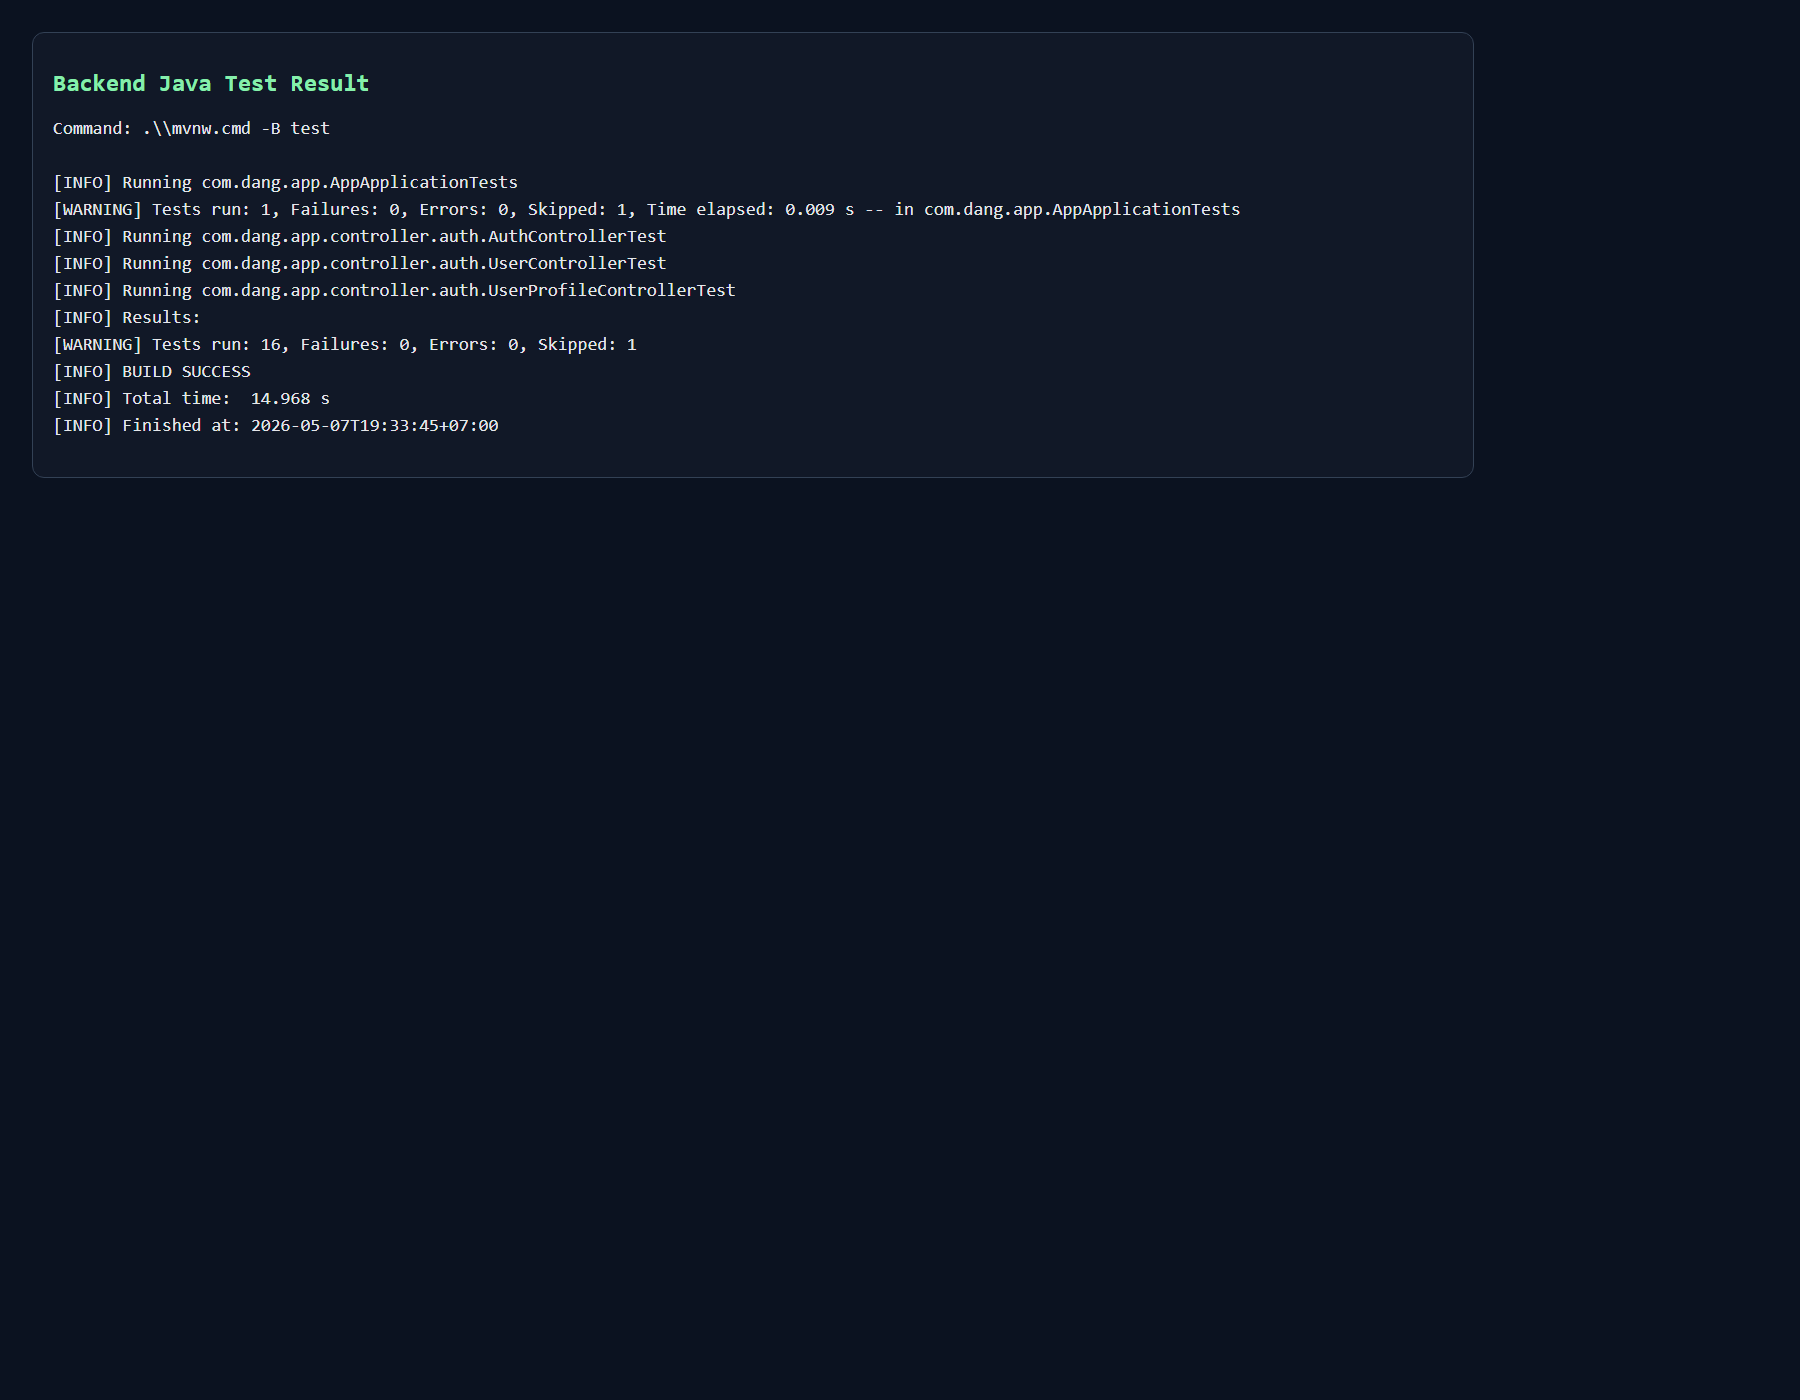
\includegraphics[width=0.95\textwidth]{images/test-shots/test-result-java.png}
    \caption{Kết quả chạy test tự động backend Java}
\end{figure}

\begin{figure}[H]
    \centering
    
\includegraphics[width=0.95\textwidth]{images/test-shots/swagger-csharp-deploy.png}
    \caption{Swagger backend C\# trên môi trường deploy}
\end{figure}

\begin{figure}[H]
    \centering
    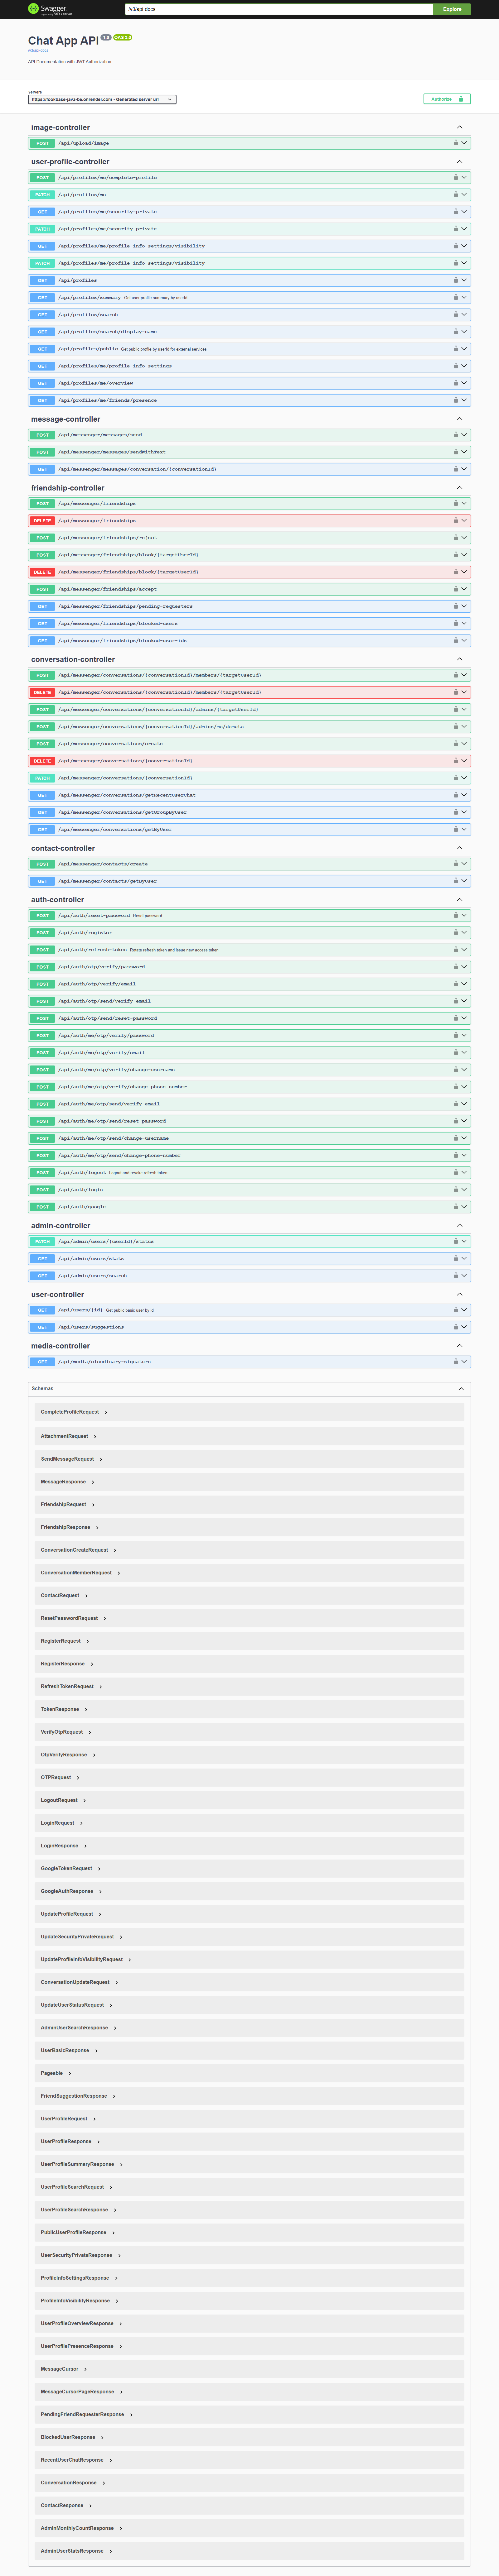
\includegraphics[width=0.95\textwidth]{images/test-shots/swagger-java-deploy.png}
    \caption{Swagger backend Java trên môi trường deploy}
\end{figure}

\begin{figure}[H]
    \centering
    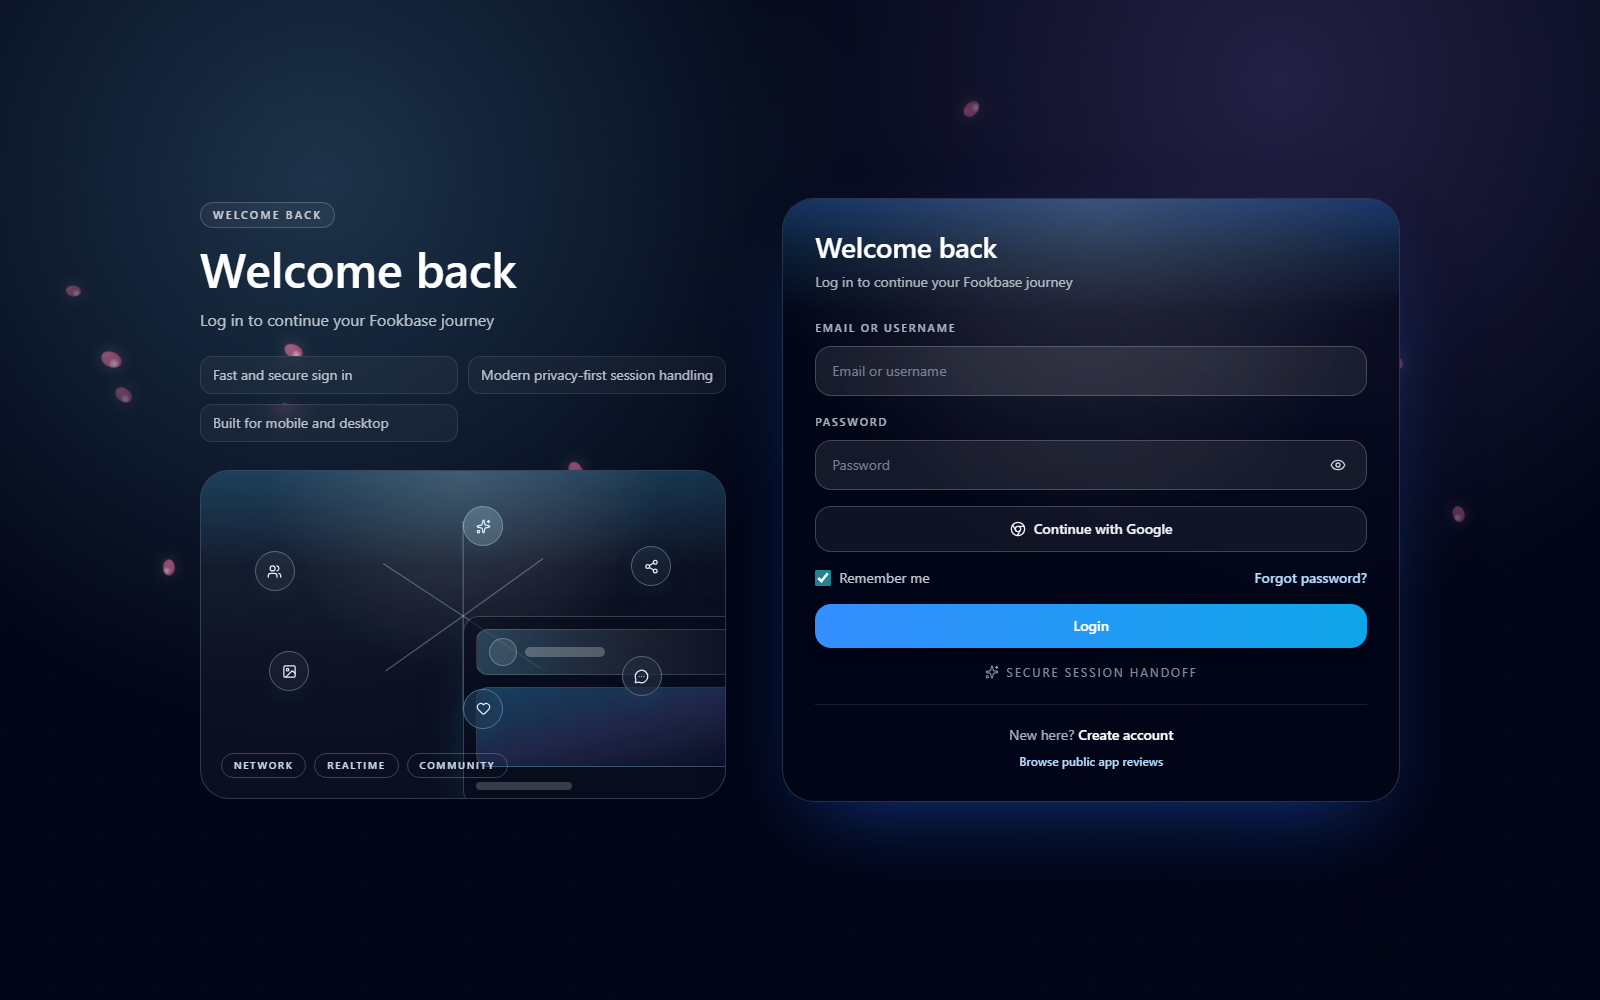
\includegraphics[width=0.9\textwidth]{images/test-shots/frontend-deploy-login.png}
    \caption{Giao diện đăng nhập frontend trên môi trường deploy}
\end{figure}

\begin{figure}[H]
    \centering
    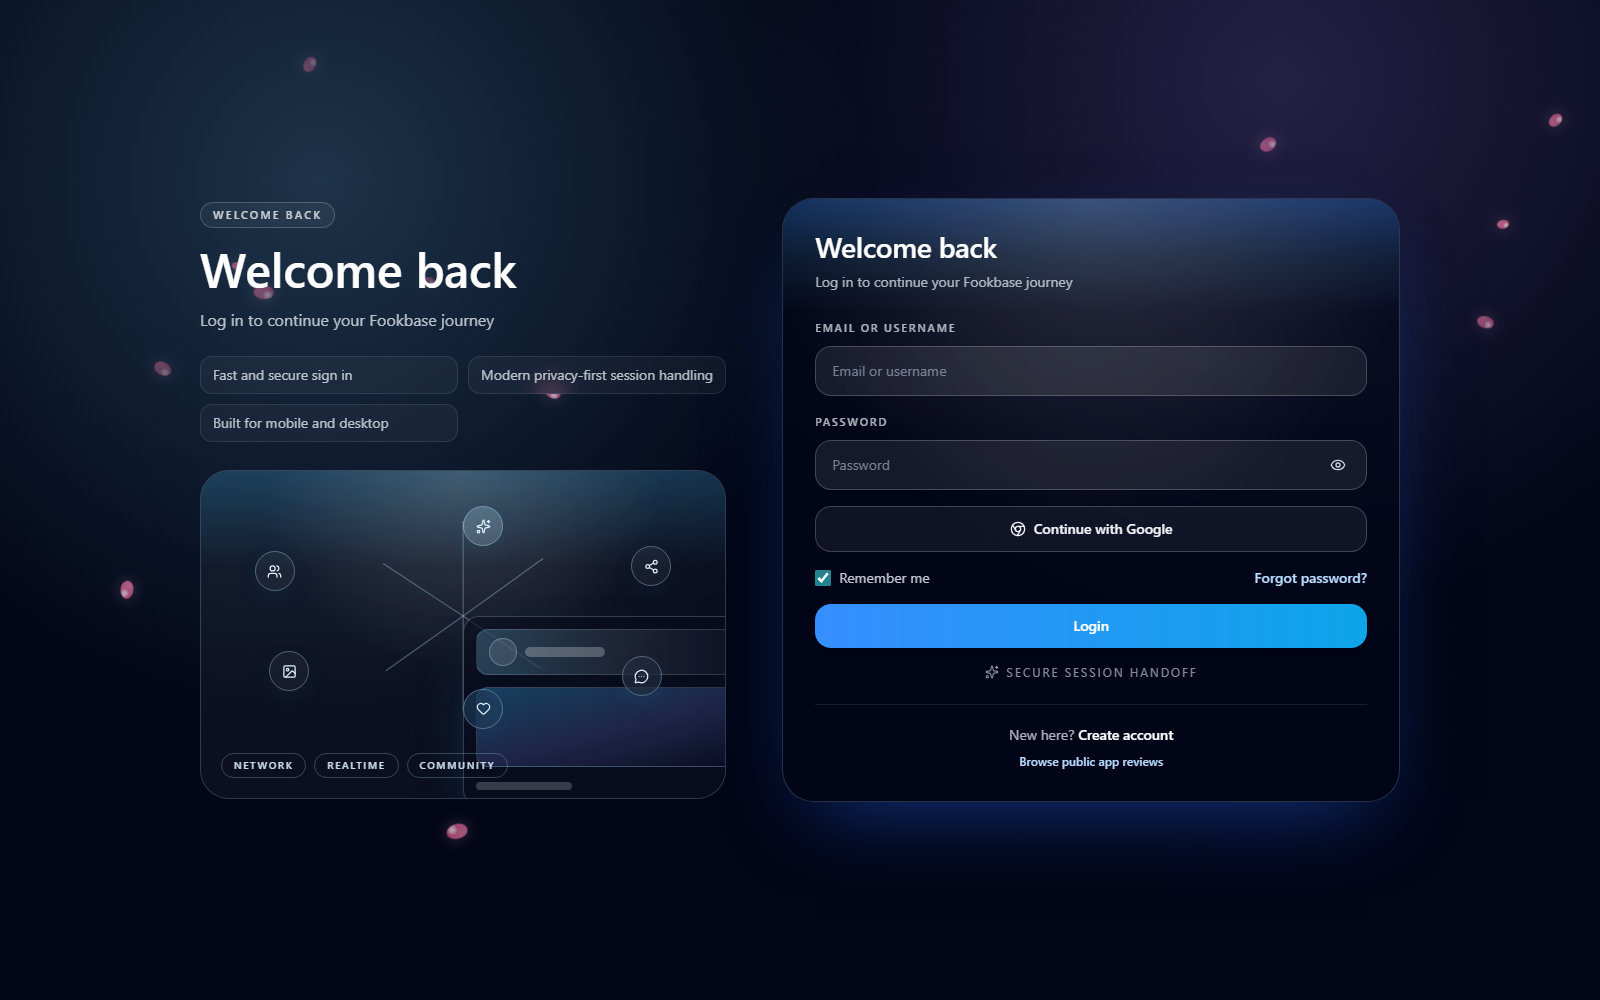
\includegraphics[width=0.9\textwidth]{images/test-shots/frontend-deploy-home.png}
    \caption{Giao diện trang chủ frontend trên môi trường deploy}
\end{figure}

\subsection{Mô tả kết quả kiểm thử}
Kết quả kiểm thử cho thấy hệ thống đã đáp ứng tốt các yêu cầu chính của đồ án: xác thực người dùng, quản lý phiên đăng nhập, hiển thị bảng tin, tạo bài viết, tương tác và truy xuất hồ sơ. Hai backend (Java và C\#) đều có bộ test tự động chạy thành công, giúp giảm rủi ro hồi quy khi chỉnh sửa mã nguồn. Trong giai đoạn tiếp theo, nhóm cần bổ sung thêm kiểm thử tải, kiểm thử bảo mật và kiểm thử tự động cho frontend để tăng độ ổn định khi số lượng người dùng tăng.

% ========================= ĐÁNH GIÁ =========================
\section{Đánh giá hệ thống}

\subsection{Ưu điểm}
\begin{itemize}
    \item Giao diện trực quan, gần với mô hình mạng xã hội thực tế.
    \item Có sự tách biệt giữa giao diện, xử lý nghiệp vụ và dữ liệu.
    \item Các chức năng chính của mạng xã hội đã được triển khai.
    \item Luồng hoạt động giữa người dùng và API rõ ràng, dễ theo dõi.
    \item Đã xây dựng kiểm thử tự động cho backend ở cả hai nền tảng: C\# (xUnit + Moq) và Java (JUnit5 + MockMvc), giúp kiểm soát hồi quy khi thay đổi mã nguồn.
    \item Kết quả chạy test ổn định: backend C\# đạt \textbf{33/33} test pass, backend Java \textbf{16} test chạy với \textbf{0 lỗi thất bại}, cho thấy độ tin cậy tốt ở lớp API.
\end{itemize}

\subsection{Hạn chế}
\begin{itemize}
    \item Chưa tối ưu toàn bộ hiệu năng hệ thống khi nhiều người dùng truy cập đồng thời.
    \item Chưa triển khai đầy đủ các cơ chế bảo mật nâng cao.
    \item Chức năng thông báo thời gian thực và nhắn tin có thể chưa hoàn thiện ở một số kịch bản biên.
    \item Kiểm thử tự động cho frontend chưa đầy đủ (chủ yếu đang kiểm thử tích hợp thủ công), nên khả năng phát hiện lỗi giao diện hồi quy còn hạn chế.
\end{itemize}

% ========================= KẾT LUẬN =========================
\section{Kết luận}

Đề tài xây dựng trang web mạng xã hội Fookbase đã giúp nhóm tiếp cận quy trình phát triển một hệ thống web hoàn chỉnh từ giao diện, xử lý API, tổ chức dữ liệu đến kiểm thử chức năng. Thông qua việc hiện thực các chức năng như đăng nhập, tạo bài viết, tương tác bài viết và quản lý hồ sơ cá nhân, nhóm đã hiểu rõ hơn về cách các thành phần trong hệ thống phối hợp với nhau để tạo nên một ứng dụng web thực tế.

Trong tương lai, hệ thống có thể được mở rộng thêm nhiều chức năng nâng cao như nhắn tin thời gian thực, thông báo realtime, chia sẻ bài viết, phân quyền chi tiết hơn, tối ưu hiệu năng và nâng cao bảo mật. Đây sẽ là nền tảng quan trọng để tiếp tục phát triển Fookbase thành một sản phẩm hoàn thiện hơn.

% ========================= TÀI LIỆU THAM KHẢO =========================
\begin{thebibliography}{9}

\bibitem{react}
React Documentation. 
\textit{Available at: https://react.dev/}

\bibitem{aspnet}
Microsoft ASP.NET Core Documentation.
\textit{Available at: https://learn.microsoft.com/aspnet/core}

\bibitem{spring}
Spring Framework Documentation.
\textit{Available at: https://spring.io/projects/spring-framework}

\bibitem{restapi}
MDN Web Docs -- HTTP.
\textit{Available at: https://developer.mozilla.org/}

\end{thebibliography}

\end{document}
